\documentclass[10pt,english]{article}
\raggedbottom
\sloppy
\usepackage{graphicx} % Required for inserting images
\usepackage{amsmath}
\usepackage{amssymb}
\usepackage{authblk}
\usepackage{algorithm}
\usepackage{algpseudocode}
\usepackage[english]{babel}
\usepackage{setspace}
\usepackage{times}
\usepackage{indentfirst}
\usepackage{titlepic}
\usepackage{comment}
\usepackage{enumitem}
\usepackage[utf8]{inputenc}
\usepackage[T5]{fontenc}
\usepackage{multirow}
\usepackage{booktabs}
\usepackage{minted}
\usepackage{hyperref}
\usepackage{charter}
\usepackage{graphicx}
\usepackage{placeins}
\usepackage{float}
\usepackage{subfig}  % For subfigure support
\usepackage[table,xcdraw]{xcolor}
\usepackage[letterpaper,top=2cm,bottom=2cm,left=2.75cm,right=2.75cm,marginparwidth=1.75cm]{geometry}
\usepackage{pgfplots}
\pgfplotsset{compat=1.18}
\usepackage{float} 
\graphicspath{ {./images/} }
\setcounter{tocdepth}{3}

% --- Global spacing shrink by 20% ---
% Put in the preamble, after \documentclass
\usepackage{calc}      % allows 0.4\length arithmetic
\usepackage{setspace}  % for line spacing
\usepackage{enumitem}  % for list spacing
\usepackage{titlesec}  % for section spacing (optional but helpful)

% 1) Line spacing (baseline)
% If you previously used \onehalfspacing or \setstretch{1.2}, reduce by 20% of that:
% Example: from 1.2 -> 0.96
\setstretch{0.4} % 0.4 × the default line spacing (tight!)
% If you were already using \setstretch{s}, replace with \setstretch{0.4*s}.

% 2) Paragraph spacing/indent
\setlength{\parskip}{.4\parskip}
\setlength{\parindent}{.4\parindent}

% 3) Displayed math spacing
\setlength{\abovedisplayskip}{.4\abovedisplayskip}
\setlength{\belowdisplayskip}{.4\belowdisplayskip}
\setlength{\abovedisplayshortskip}{.4\abovedisplayshortskip}
\setlength{\belowdisplayshortskip}{.4\belowdisplayshortskip}

% 4) Floats (figures/tables) spacing
\setlength{\textfloatsep}{.4\textfloatsep}
\setlength{\floatsep}{.4\floatsep}
\setlength{\intextsep}{.4\intextsep}
\setlength{\dbltextfloatsep}{.4\dbltextfloatsep}
\setlength{\dblfloatsep}{.4\dblfloatsep}

% 5) Lists spacing (itemize/enumerate/description)
\setlist{itemsep=.2\itemsep, topsep=.2\topsep, parsep=.2\parsep, partopsep=.2\partopsep}

% 6) Section heading spacing (before/after)
% Adjust all levels uniformly; tweak if needed.
\titlespacing*{\section}{0pt}{.4\baselineskip}{.4\baselineskip}
\titlespacing*{\subsection}{0pt}{.4\baselineskip}{.4\baselineskip}
\titlespacing*{\subsubsection}{0pt}{.4\baselineskip}{.4\baselineskip}

% (Optional) Tighten captions slightly (requires caption package)
% \usepackage[skip=.4\baselineskip]{caption}
\pgfplotsset{
  colormap={myblues}{
    rgb255(0cm)=(239,243,255)
    rgb255(1cm)=(8,69,148)
  }
}

\begin{document}
 
\begin{titlepage}
\begin{center}

\textsc{\large \textcolor{black}{\textbf{HANOI UNIVERSITY OF SCIENCE AND TECHNOLOGY }}}\\[0.5cm]

{\huge \Large \uppercase{School of Information Communication Technology} \\[1cm] }

\includegraphics[scale=0.13]{logo-soict-hust-1.png}\\[1cm]
\textsc{\Large \textbf{Project report:}}\\[0.4cm]	

\rule{\linewidth}{0.7mm} \\[0.4cm]
{ \huge \bfseries\color{black!70!black} Sentiment Analysis for Video Game Reviews \\[0.4cm] }
\rule{\linewidth}{0.7mm} \\[1cm]

\color{black!80!black}{\large \textbf{\textit{Supervised by}:}}\\[0.4cm]

\begin{tabular}{l}
\large  Ph.D. Nguyen Kiem Hieu  \\[1cm]
\end{tabular}

\color{black!80!black}{\large \textbf{\textit{Presented by}:}}\\[0.4cm]
\color{black}
\begin{tabular}{l}

\large Au Trung Phong - 20225455 \\[0.4cm]
\large Nguyen Nam Khanh - 20225448 \\[0.4cm]
\large Vu Duc Minh - 20225514 \\[0.4cm]
\large Tran Sy Minh Quan - 20225521 \\[0.4cm]
\large Bui Van Huy - 20225497 \\[0.4cm]

\end{tabular}

\vfill

{\large \color{black!80!black}{\textbf{Hanoi - Vietnam}}\\[0.2cm] \color{blue!90!black}2025}

\end{center}
\end{titlepage}
\setstretch{1.5}


\tableofcontents

\section{Introduction}

\subsection{Context and Motivation}
The video game industry has evolved into a dominant force in global entertainment, surpassing both the film and music industries in revenue. According to recent market intelligence by Newzoo, the global games market is projected to generate approximately \$187.7 billion in 2024, with the number of active players worldwide reaching nearly 3.4 billion \cite{newzoo2024}. Unlike passive forms of media, gaming is deeply interactive, fostering passionate communities that generate massive volumes of feedback across social media, forums, and review aggregators.

This explosion of User-Generated Content (UGC) has fundamentally shifted how games are marketed and consumed. Research indicates that up to 93\% of consumers find UGC helpful when making purchasing decisions, and approximately 70\% of gamers consult reviews or ratings before buying a title \cite{stackla2019}. Platforms like Metacritic have emerged as central hubs for this ecosystem, where a game's aggregate score (Metascore) can determine its commercial success, influence stock prices, and even dictate the financial bonuses of development teams \cite{wingfield2007}.

However, the sheer velocity and volume of this data present a significant challenge. A single popular game release can generate tens of thousands of reviews in a matter of days. These reviews range from detailed, multi-paragraph critiques to slang-filled one-liners (e.g., ``This game is buggy but the combat is fire''). Manual analysis of this unstructured text is impossible at scale. Consequently, automated ``Opinion Mining'' (or Sentiment Analysis) has transitioned from an academic curiosity to an industrial necessity. It allows developers and publishers to monitor brand health, identify critical bugs, and quantify player satisfaction in real-time.


\subsection{Problem Statement}
The core technical problem addressed in this project is the automated classification of sentiment in unstructured game reviews. While general sentiment analysis is a well-studied field, the gaming domain presents unique linguistic challenges that general-purpose models often fail to capture.

\paragraph{Formal Problem Definition}
Given a dataset $\mathcal{D} = \{(x_i, y_i)\}_{i=1}^{N}$ of $N$ game reviews, where each review $x_i$ is a sequence of tokens $x_i = (w_1, w_2, \ldots, w_{|x_i|})$ and $y_i \in \mathcal{Y}$ is its corresponding sentiment label from the set $\mathcal{Y} = \{\text{Positive}, \text{Mixed}, \text{Negative}\}$ with $|\mathcal{Y}| = 3$, the objective is to learn a classification function:

\begin{equation}
f: \mathcal{X} \rightarrow \mathcal{Y}, \quad \text{where } |\mathcal{Y}| = 3
\end{equation}

\noindent that maps an arbitrary review text $x \in \mathcal{X}$ to one of the three sentiment classes $y \in \mathcal{Y}$, minimizing the expected classification error:

\begin{equation}
\mathcal{L}(f) = \mathbb{E}_{(x,y) \sim \mathcal{D}} \left[ \mathbb{1}(f(x) \neq y) \right]
\end{equation}

\noindent where $\mathbb{1}(\cdot)$ is the indicator function that equals 1 when the condition is true and 0 otherwise.

\paragraph{Problem Characteristics}
\begin{itemize}
    \item \textbf{Input:} A dataset of natural language reviews collected from online gaming platforms. These inputs are characterized by high variance in length, informal grammar, and heavy usage of domain-specific terminology (e.g., ``nerf,'' ``buff,'' ``grindy,'' ``framerate,'' ``pay-to-win'').
    \item \textbf{Output:} A predicted sentiment label for each review (Positive, Mixed, Negative).
    \item \textbf{Key Challenges:}
    \begin{enumerate}
        \item \textbf{Domain Adaptation:} Standard NLP models trained on formal corpora (like Wikipedia) often misinterpret gaming slang. For instance, the word ``sick'' is positive in a gaming context, whereas ``broken'' can refer to a bug (negative) or an overpowered mechanic (context-dependent).
        \item \textbf{Data Quality:} User-generated game reviews are often polarized or sarcastic, complicating sentiment detection.
        \item \textbf{Scalability:} The solution must be efficient enough to process large datasets without excessive computational overhead.
    \end{enumerate}
\end{itemize}

\subsection{Project Objectives}
The primary goal of this capstone project is to develop a comprehensive pipeline for gaming sentiment analysis, spanning from raw data collection through model evaluation and public release. The specific objectives are defined as follows:

\begin{enumerate}
    \item \textbf{Dataset Construction:} To create a valuable benchmark dataset by scraping, aggregating, and cleaning thousands of reviews from Metacritic. This involves using advanced web scraping tools to handle dynamic content and filtering specifically for English-language feedback.
    
    \item \textbf{Methodological Comparison:} To implement and strictly evaluate three distinct modeling approaches to understand the trade-off between complexity and performance:
    \begin{itemize}
        \item \textbf{Baseline Model (LSTM):} Implementing a Long Short-Term Memory network with a standard trainable embedding layer. This serves as a conventional baseline to measure performance improvements without reliance on pre-trained external vectors.
        \item \textbf{Fine-tuning Large Language Model Approach (RoBERTa):} Fine-tuning a RoBERTa transformer model to leverage deep contextual understanding and attention mechanisms.
        \item \textbf{Dense Embedding with Machine Learning Approach (EmbeddingGemma + XGBoost):} Proposing a modern approach that combines state-of-the-art dense vector representations (EmbeddingGemma-300M) with gradient boosting (XGBoost) to achieve high accuracy with lower training costs.
    \end{itemize}
    
    \item \textbf{Performance Analysis and Model Release:} To provide a comprehensive evaluation using standard metrics including per-class and aggregate measures (Accuracy, Precision, Recall, F1-Score, Confusion Matrix), along with efficiency metrics (Training Time, Throughput) to analyze which architecture offers the best performance for the specific nuances of game reviews while maintaining practical computational feasibility. Additionally, to release all trained models and code artifacts to the HuggingFace Hub for reproducibility, accessibility, and potential integration into downstream applications.
\end{enumerate}

\section{Background}


\subsection{Sentiment Analysis in Domain-Specific Contexts}
Sentiment Analysis (SA), or opinion mining, is a pivotal task in Natural Language Processing (NLP) that aims to determine the polarity of subjective text. While general SA models have achieved significant success on standard datasets like IMDb (movies) or Yelp (restaurants), they often struggle when applied to the gaming domain due to its unique linguistic characteristics.

One major challenge in gaming reviews is the high prevalence of domain-specific slang and evolving terminology. Research by Panwar and Bhatnagar \cite{panwar2022sentiment} highlights that generic sentiment lexicons fail to capture the nuanced meaning of terms like ``frag'' (kill), ``grind'' (repetitive gameplay), or ``camp'' (waiting for enemies), which can be neutral or negative depending on context. Furthermore, gaming communities frequently employ sarcasm and irony, which remain persistent hurdles for traditional machine learning models. A survey by Hussein \cite{hussein2018survey} identifies sarcasm detection as a critical bottleneck, noting that gamers often use ostensibly positive words (e.g., ``Great job crashing every 5 minutes'') to express severe dissatisfaction.

Another significant issue is the structural complexity of game reviews. Unlike product reviews that focus on a single tangible object, game reviews often discuss multiple heterogeneous aspects such as graphics, gameplay mechanics, story, and technical performance. Viggiato et al. \cite{viggiato2021causes} demonstrated that off-the-shelf sentiment classifiers trained on non-gaming data perform poorly on game reviews (achieving AUC scores as low as 0.53), largely because they cannot distinguish between sentiment directed at a specific buggy feature versus the overall game experience. This necessitates the development of domain-adapted models capable of understanding these specific contexts.

\subsection{Recurrent Neural Networks and Long Short-Term Memory}

\paragraph{Motivation}
The LSTM approach serves as a \textbf{conventional baseline} for this project, representing the traditional deep learning paradigm before the widespread adoption of pre-trained language models. By training an LSTM network from scratch with randomly initialized embeddings, we establish a performance benchmark that relies solely on the domain-specific training data without leveraging external pre-trained knowledge. This allows us to quantify the incremental value provided by modern pre-trained architectures (RoBERTa) and hybrid approaches (EmbeddingGemma + XGBoost). Furthermore, LSTMs remain relevant in resource-constrained scenarios where model interpretability and deployment simplicity are prioritized over absolute performance.

Recurrent Neural Networks (RNNs) are designed to process sequential data but often struggle with the vanishing gradient problem, limiting their ability to learn long-term dependencies in text. To address this, Hochreiter and Schmidhuber \cite{hochreiter1997long} introduced Long Short-Term Memory (LSTM) networks, which utilize gating mechanisms to selectively retain or discard information over long sequences.

The information flow within an LSTM cell is regulated by the following transition functions:

\begin{equation}
\begin{aligned}
f_t &= \sigma(W_f \cdot [h_{t-1}, x_t] + b_f) & \text{(Forget Gate)} \\
i_t &= \sigma(W_i \cdot [h_{t-1}, x_t] + b_i) & \text{(Input Gate)} \\
C_t &= f_t \odot C_{t-1} + i_t \odot \tanh(W_C \cdot [h_{t-1}, x_t] + b_C) & \text{(Cell State)} \\
o_t &= \sigma(W_o \cdot [h_{t-1}, x_t] + b_o) & \text{(Output Gate)} \\
h_t &= o_t \odot \tanh(C_t) & \text{(Hidden State)}
\end{aligned}
\end{equation}

\noindent where $\sigma$ denotes the sigmoid function and $\odot$ denotes element-wise multiplication.

To capture context from both preceding and succeeding words, this project utilizes a Bidirectional LSTM (BiLSTM), which processes input sequences in both directions. The specific architectural implementation for this study is adapted from Dhanjal and Sinha \cite{mahadevaswamy2023sentiment}, who demonstrated the efficacy of BiLSTM networks for sentiment classification tasks.


\subsection{Large Language Models (LLMs) and Fine-tuning Strategies}

\paragraph{Motivation}
The RoBERTa approach represents the \textbf{state-of-the-art paradigm} in transfer learning for NLP tasks. Gaming reviews present unique challenges, including domain-specific slang (``nerf,'' ``grind,'' ``meta''), sarcasm, and complex multi-aspect opinions, which require deep contextual understanding beyond what surface-level features can capture. By fine-tuning a pre-trained Transformer model, we leverage billions of tokens of linguistic knowledge encoded during pre-training, then adapt this understanding to the gaming domain through task-specific fine-tuning. This approach is expected to achieve the highest classification performance due to its ability to model long-range dependencies, contextual nuances, and subtle semantic distinctions. However, this performance comes at the cost of substantial computational requirements and longer training times, making it important to evaluate whether the performance gains justify the resource investment.

While LSTMs improved sequential modeling, they remain constrained by their sequential nature, which precludes parallelization and limits the retention of context in very long sequences. The introduction of the Transformer architecture by Vaswani et al. \cite{vaswani2017attention} revolutionized NLP by utilizing the \textbf{Self-Attention Mechanism}, allowing models to weigh the importance of all words in a sentence simultaneously, regardless of their distance from each other.

\subsubsection{RoBERTa Architecture}
For this project, we utilize \textbf{RoBERTa} (Robustly Optimized BERT Pretraining Approach), introduced by Liu et al. \cite{liu2019roberta}. RoBERTa is an encoder-only Transformer model that builds upon BERT's architecture but introduces critical optimizations that make it highly effective for complex sentiment analysis:

\begin{itemize}
    \item \textbf{Dynamic Masking:} Unlike BERT, which masks tokens once during data preprocessing, RoBERTa generates a unique masking pattern for every training sequence, effectively augmenting the data and preventing the model from overfitting to specific masking patterns.
    \item \textbf{Removal of Next Sentence Prediction (NSP):} Research indicated that the NSP objective used in BERT was unnecessary for performance; removing it allows RoBERTa to focus entirely on the Masked Language Modeling (MLM) objective.
    \item \textbf{Larger Contexts and Batches:} RoBERTa is trained on significantly larger mini-batches and more diverse datasets, resulting in strictly better performance on downstream tasks compared to the original BERT.
\end{itemize}

\subsubsection{Fine-Tuning Strategy}
Instead of training a Transformer from scratch, which requires massive computational resources, we employ \textbf{Transfer Learning}. We initialize the model with pre-trained weights learned from a massive corpus and fine-tune it on our game review dataset.

Mathematically, given the final hidden vector $h_{CLS}$ corresponding to the special classification token (representing the entire sentence), the probability distribution over the sentiment classes $y$ is computed by passing $h_{CLS}$ through a linear classification head:

\begin{equation}
P(y|x) = \text{softmax}(W_{task} \cdot h_{CLS} + b_{task})
\end{equation}

\noindent where $W_{task}$ and $b_{task}$ are the parameters specific to the sentiment classification layer that are updated during fine-tuning, while the underlying RoBERTa weights are fine-tuned at a lower learning rate.

\subsection{Dense Vector Representations and Gradient Boosting}

\paragraph{Motivation}
The EmbeddingGemma + XGBoost pipeline represents a \textbf{pragmatic hybrid approach} that balances performance with computational efficiency. While fine-tuning large language models yields excellent results, it requires significant GPU resources and time for every training iteration. By decoupling semantic understanding (via pre-trained embeddings) from classification (via gradient boosting), we achieve several strategic advantages: (1) embeddings can be computed once and reused across multiple experiments, (2) XGBoost training is orders of magnitude faster than Transformer fine-tuning, enabling rapid hyperparameter exploration, and (3) the model footprint is dramatically smaller, facilitating deployment in resource-constrained production environments. This approach tests the hypothesis that modern embedding models have become sufficiently powerful that a sophisticated classical classifier can match or approach the performance of end-to-end neural models, while offering superior training efficiency and interpretability through feature importance analysis.

While end-to-end deep learning models like RoBERTa are powerful, they are computationally expensive. An alternative approach is to decouple the \textit{understanding} of text from the \textit{classification} task. This involves using a pre-trained Large Language Model purely as a feature extractor to generate high-quality ``embeddings,'' which are then fed into a highly efficient structured data classifier.

\subsubsection{Semantic Embeddings via EmbeddingGemma}
Text embeddings map discrete text sequences into a continuous vector space $$\mathbb{R}^d$$, where $d$ is the dimension of the embedding (typically $d=768$ for this model). In this space, semantic similarity is preserved as geometric proximity; reviews with similar meanings are located closer together.

For this project, we utilize \textbf{EmbeddingGemma (google/embeddinggemma-300m)} \cite{vera2025embeddinggemma}. This model is a compact, 300-million-parameter embedding model derived from the Gemma 3 family. Unlike larger monolithic models, EmbeddingGemma is optimized for resource-constrained environments while maintaining state-of-the-art performance. It employs contrastive learning and Matryoshka Representation Learning to produce robust dense vectors across over 100 languages.

We selected this model for two primary reasons:
\begin{enumerate}
    \item \textbf{Resource Efficiency:} With only 300M parameters, the model fits comfortably within the memory constraints of the Kaggle environment (specifically the NVIDIA Tesla P100 16GB GPU), allowing for larger batch sizes and fast inference.
    \item \textbf{High Performance:} Despite its small size, it achieves competitive rankings on the Massive Text Embedding Benchmark (MTEB), ranking \textbf{11th in the Borda count} and \textbf{16th in Classification tasks} \cite{enevoldsen2025mmtebmassivemultilingualtext}.
\end{enumerate}

Given an input sentence $x$, the embedding model $E$ produces a fixed-size vector $v$:

\begin{equation}
v = E(x), \quad v \in \mathbb{R}^d
\end{equation}

\noindent This vector $v$ serves as a dense numerical representation of the review's semantic content, capturing nuances that simple Bag-of-Words models miss.

\subsubsection{Gradient Boosting with XGBoost}
Once the text is converted into dense vectors, the sentiment analysis task becomes a standard tabular classification problem. We employ \textbf{XGBoost (eXtreme Gradient Boosting)} \cite{chen2016xgboost}, an ensemble learning method based on decision trees.

XGBoost constructs a strong classifier by sequentially adding ``weak'' learners (decision trees). Each new tree is trained to correct the residual errors made by the previous ensemble of trees. The prediction $\hat{y}_i$ for a given instance $i$ at step $K$ is the sum of predictions from $K$ trees:

\begin{equation}
\hat{y}_i = \sum_{k=1}^{K} f_k(v_i), \quad f_k \in \mathcal{F}
\end{equation}

\noindent where $\mathcal{F}$ is the space of regression trees. XGBoost is particularly chosen for its ability to handle dense numerical features effectively, its regularization techniques to prevent overfitting, and its computational efficiency compared to fine-tuning massive Transformers.

\section{Methodology}


\subsection{Phase 1: Data Acquisition}
% - Source: Metacritic.
% - Tools: Scrapy framework integrated with Playwright for handling dynamic JavaScript content.
% - Process:
%   - Game discovery logic (pagination, platform filtering).
%   - Review scraping (text, score, user, date).

The foundation of this project is the construction of a novel, domain-specific dataset derived from Metacritic, a leading review aggregator for the gaming industry. The data acquisition process was designed to be robust, scalable, and capable of handling dynamic web content.

\subsubsection{Game Discovery Module}
The first step involved identifying a diverse list of games to ensure the dataset covers various genres, platforms, and time periods. We implemented a custom Python script which employs standard web scraping techniques. This script iterates through Metacritic's game listings, utilizing pagination handling to traverse multiple pages of search results.

For efficiency and simplicity, the discovery module extracts the URL-safe identifier for each game encountered. This serves as a unique key used to construct the direct link to each game's review page.

The output is stored as plain text files, with one identifier per line (e.g., ``the-legend-of-zelda-ocarina-of-time''). To manage large-scale discovery operations, the script supports splitting output across multiple files, enabling parallel processing in subsequent scraping phases. The discovered game identifiers serve as the input queue for the review scraper module.

\subsubsection{Review Scraping Engine}
To extract the actual review content, we developed a sophisticated scraping engine using \textbf{Scrapy}, a high-level web crawling framework, integrated with \textbf{Playwright}. This combination was essential because Metacritic relies heavily on JavaScript to render user reviews dynamically. Standard HTTP requests would fail to load the full content.

The spider operates as follows:
\begin{enumerate}
    \item \textbf{Request Handling:} It accepts the list of discovered game slugs and processes them sequentially with configurable delays between games.
    \item \textbf{Dynamic Rendering:} Playwright launches a headless browser instance to render the DOM (Document Object Model) fully, triggering the necessary JavaScript events to load all reviews.
    \item \textbf{Progressive Loading:} To load all available reviews, the engine automatically scrolls through the page and clicks ``Load More'' buttons, with timeout protection and duplicate detection to prevent infinite loops.
    \item \textbf{Data Extraction:} The spider parses the rendered HTML to extract comprehensive review and game metadata:
\begin{itemize}
    \item \textbf{Review Text:} The body of the user's comment.
    \item \textbf{User Score:} The numerical rating (0-10 scale, normalized to 0-100 for consistency).
    \item \textbf{Review Category:} Extracted directly from Metacritic's color-coded sentiment badges: positive (green, $\geq$75), mixed (yellow, 50-74), or negative (red, $<$50), which represent Metacritic's domain-expert classification of review sentiment.
    \item \textbf{Review Platform:} The specific platform for which the review was written, extracted at the individual review level from the rendered page.
    \item \textbf{Date:} The submission date of the review.
    \item \textbf{Username:} Identifier for the reviewer.
    \item \textbf{Game Metadata:} Title, platform, metascore, release date, genre, developer, and publisher for contextual analysis.
    \end{itemize}
    \item \textbf{Incremental Storage and Recovery:} Reviews are incrementally appended after each game completes, with progress tracking to enable automatic resumption if interrupted.
    \item \textbf{Rate Limiting:} To adhere to ethical scraping guidelines and avoid server overload, we configured inter-game delays, enabled auto-throttling, and limited concurrent requests, ensuring a respectful request pace that adapts to server response times.
    \end{enumerate}
The raw output is saved as JSON Lines files, with each review stored as a separate JSON object on its own line, facilitating efficient line-by-line processing in subsequent stages.

\subsection{Phase 2: Data Preparation}
Raw web data is inherently noisy and unstructured. Phase 2 focused on transforming the raw collection into a clean, machine-learning-ready benchmark dataset.

\subsubsection{Aggregation and Cleaning}
We developed an aggregation pipeline to consolidate the scattered data files from Phase 1. Key preprocessing steps included:
\begin{itemize}
    \item \textbf{Language Filtering:} Since the scope of this project is English sentiment analysis, we applied the \texttt{langdetect} library to identify and retain only English reviews. While individual reviews may contain occasional non-English words (e.g., game titles or character names), the library's n-gram-based detection ensures the overall text is predominantly English, maintaining vocabulary consistency for the embedding layers and preventing multilingual interference.
    \item \textbf{Deduplication:} Duplicate reviews (e.g., spam or multiple scrapes of the same page) were identified via normalized text comparison and removed to prevent data leakage between training and test sets.
    \item \textbf{Field Selection:} From the rich metadata collected during scraping, we extracted only the essential fields for sentiment analysis: review text and review category. User scores, while collected as part of comprehensive dataset construction, were not utilized in the classification task but remain available for potential future correlation studies or multi-task learning experiments.
\end{itemize}
Note that text normalization (whitespace standardization) was performed during the scraping phase itself, ensuring clean input to the aggregation pipeline.

\subsubsection{Sentiment Labels}
Sentiment labels were directly extracted from Metacritic's platform during Phase 1. Metacritic employs a three-tier classification system that color-codes user reviews based on their scores:
\begin{itemize}
    \item \textbf{Positive:} Reviews marked with green badges.
    \item \textbf{Mixed:} Reviews marked with yellow badges, representing reviews with balanced or ambivalent sentiment.
    \item \textbf{Negative:} Reviews marked with red badges.
\end{itemize}
These pre-labeled categories were scraped directly from the HTML structure, eliminating the need for manual annotation or score-based heuristics. This approach ensures that our labels align precisely with Metacritic's domain expertise in game review sentiment classification. All three categories were retained in the final dataset to enable both binary (positive vs. negative) and ternary (including mixed) classification experiments.

\subsubsection{Dataset Splitting}
To guarantee rigorous evaluation, the processed dataset was deterministically split using a fixed random seed into three subsets:
\begin{itemize}
    \item \textbf{Training Set (80\%):} Used for model parameter updates during backpropagation.
    \item \textbf{Validation Set (10\%):} Used for hyperparameter tuning, early stopping, and model selection during training.
    \item \textbf{Test Set (10\%):} Held out completely until the final evaluation phase to report unbiased performance metrics.
\end{itemize}
The splitting was performed after shuffling to ensure random distribution across all sentiment categories and prevent temporal or game-specific biases. The final dataset was formatted for the HuggingFace Hub, enabling seamless integration with modern NLP libraries such as Transformers and Datasets.

\subsection{Phase 3: Model Training}
The final phase involves the development and evaluation of three distinct sentiment classification models. The training pipeline implements a rigorous two-phase strategy to ensure optimal hyperparameter selection and unbiased performance evaluation.

\textbf{Two-Phase Training Strategy: }
All models follow a systematic approach to hyperparameter optimization and final model training, ensuring reproducible and unbiased performance assessment.

\paragraph{Phase 1: Grid Search (Hyperparameter Exploration)}
The first phase conducts exhaustive hyperparameter search using a subset of the training data to efficiently identify optimal model configurations:
\begin{itemize}
    \item \textbf{Data Partitioning:} Grid search uses only training and validation splits (typically 10\% for computational efficiency). The test set remains completely untouched to prevent information leakage.
    \item \textbf{Evaluation Protocol:} Models are trained on the training subset and evaluated exclusively on the validation set using F1-macro score as the primary optimization metric, ensuring equal importance for all sentiment categories (positive, mixed, negative).
    \item \textbf{Hyperparameter Space:} Each model explores its relevant hyperparameter space (learning rates, regularization strengths, architectural choices) with results automatically saved to \texttt{best\_config.txt}. These exploration models are not uploaded to HuggingFace Hub.
    \item \textbf{Output:} The configuration achieving the highest validation F1-macro score is identified and logged, along with comprehensive grid search results in \texttt{gridsearch\_results.json}.
\end{itemize}

\paragraph{Phase 2: Final Training (Production-Ready Model)}
Using the optimal hyperparameters discovered in Phase 1, the second phase trains the final production-ready model:
\begin{itemize}
    \item \textbf{Full Dataset Training:} The model is retrained on 100\% of the training data (not the 10\% subset) with the best hyperparameters, maximizing the model's exposure to training examples.
    \item \textbf{Test Set Evaluation:} The held-out test set is evaluated for the \textbf{first and only time} during this phase, providing unbiased performance metrics that accurately reflect the model's generalization capability on truly unseen data.
    \item \textbf{Model Release:} The final trained model, along with all necessary artifacts (tokenizers, label encoders, configuration files, and training logs), is saved locally and uploaded to the HuggingFace Hub for reproducibility, sharing, and potential integration into downstream applications or further development.
\end{itemize}

This two-phase methodology ensures that hyperparameter selection is both data-driven and computationally efficient, while final performance reporting maintains scientific rigor through strict test set isolation.

\subsubsection{Baseline Model: Bidirectional LSTM}
% - Architecture: Trainable Embedding Layer -> LSTM layers -> Dense classification head.
% - Embedding Strategy: Utilizing a standard nn.Embedding layer (randomly initialized and learned during training) to capture domain-specific vocabulary directly from the dataset.
% - Purpose: To establish a conventional benchmark for performance without reliance on external pre-trained static vectors.
To establish a robust benchmark for sentiment analysis without relying on external pre-trained models, we constructed a deep learning architecture based on the Bidirectional Long Short-Term Memory (Bi-LSTM) network. As described in \cite{mahadevaswamy2023sentiment}, this architecture extends the traditional RNN by processing sequence data in both forward and backward directions, allowing the model to capture context from both past and future states, thereby effectively handling long-term dependencies in text.

\paragraph{Data Preprocessing and Tokenization}
The text data is processed using a custom \texttt{SimpleTokenizer} designed to build a domain-specific vocabulary directly from the training corpus.
\begin{itemize}
    \item \textbf{Vocabulary Construction:} The vocabulary is built by counting word frequencies in the training set and selecting the top 73,738 most common words ($|V| = 73,738$).
    \item \textbf{Sequence Formatting:} Each review is tokenized, converted to integer indices, and standardized to a fixed length of $L=200$ tokens. Sequences shorter than this limit are padded with zeros (index 0), while longer sequences are truncated.
    \item \textbf{Label Encoding:} Target labels are encoded into integer format (e.g., negative $\rightarrow$ 0, mixed $\rightarrow$ 1, positive $\rightarrow$ 2) using a Label Encoder fitted on the training data.
\end{itemize}

\paragraph{Network Architecture}
The model architecture consists of four primary components arranged sequentially:
\begin{enumerate}
    \item \textbf{Embedding Layer:} The input layer is a trainable embedding matrix $E \in \mathbb{R}^{|V| \times d_{emb}}$, where the embedding dimension $d_{emb}$ is set to 128. This layer learns dense vector representations for each token during the training process.
    \item \textbf{Stacked Bi-LSTM Layers:} We employ a stack of 2 Bidirectional LSTM layers. Each layer has a hidden dimension of $h_{dim}=128$ per direction. Consequently, the output at each timestep is the concatenation of the forward and backward hidden states, resulting in a feature vector of size 256 ($128 \times 2$).
    \item \textbf{Fully Connected Classification Head:} The extracted features (the final hidden states) are passed through a series of dense layers with Rectified Linear Unit (ReLU) activation to perform classification. The dimensionality reduction proceeds as follows:
    \[ 256 \xrightarrow{FC1} 64 \xrightarrow{FC2} 64 \xrightarrow{FC3} 16 \xrightarrow{Output} N_{classes} \]
    \item \textbf{Regularization:} To prevent overfitting, Dropout regularization with a rate of $p=0.5$ is applied after the LSTM layers and between each fully connected layer.
\end{enumerate}
The total number of trainable parameters for this configuration is approximately 10.2 million.

\paragraph{Training Configuration}
The model training follows a two-stage approach: hyperparameter optimization via grid search, followed by full-scale training with the optimal configuration. Both stages share common training infrastructure detailed in Table~\ref{tab:lstm_params}.

\begin{table}[h]
\centering
\caption{Common Hyperparameters for LSTM Training}
\label{tab:lstm_params}
\begin{tabular}{ll}
\hline
\textbf{Parameter} & \textbf{Value} \\ \hline
Embedding Dimension & 128 \\
Hidden Dimension (per direction) & 128 \\
LSTM Layers & 2 (Bidirectional) \\
Dropout Rate & 0.5 \\
Max Sequence Length & 200 tokens \\
Vocabulary Size & 73,738 \\
FC Architecture & $256 \rightarrow 64 \rightarrow 64 \rightarrow 16 \rightarrow N_{classes}$ \\
Batch Size & 64 \\
Epochs & 20 \\
Optimizer & Adam \\
Loss Function & NLLLoss (3-class) \\
\hline
\end{tabular}
\end{table}

\paragraph{Model Selection}
For each run, choose the best F1-Macro model during validation step for the final evaluation at the end of training.

\textbf{Stage 1: Grid Search for Learning Rate Optimization.}
To identify the optimal learning rate while maintaining computational efficiency, we conduct a grid search on a 10\% subset of the training data:
\begin{itemize}
    \item \textbf{Search Space:} Six learning rate candidates: $\eta \in \{10^{-5}, 5 \times 10^{-5}, 10^{-4}, 5 \times 10^{-4}, 10^{-3}, 5 \times 10^{-3}\}$.
    \item \textbf{Validation Frequency:} Every 250 training steps (adapted for smaller dataset).
    \item \textbf{Selection Metric:} Macro-averaged F1 score on the validation set, ensuring balanced performance across all sentiment classes (negative, mixed, positive).
\end{itemize}

\textbf{Stage 2: Final Training with Optimal Configuration.}
Using the best learning rate $\eta^*$ identified in Stage 1, we train on the complete dataset (100\% of training data) with validation for every 500 steps.


\subsubsection{Proposed Approach 1: Fine-Tuned RoBERTa}

To capture the deep semantic context required for understanding game reviews, we employed the \textbf{RoBERTa} (Robustly Optimized BERT Pretraining Approach) architecture. Specifically, we utilized the \texttt{FacebookAI/roberta-base} variant, which consists of a 12-layer bidirectional Transformer encoder with 125M parameters. Unlike the standard BERT model, RoBERTa is pre-trained with dynamic masking and without the Next Sentence Prediction (NSP) objective, making it particularly effective for downstream sequence classification tasks where context density varies.

\paragraph{Network Architecture}
We leveraged the pre-trained \texttt{roberta-base} model from HuggingFace's Transformers library \cite{facebookai_roberta_base}. The architecture consists of:
\begin{itemize}
    \item \textbf{Embedding Layer:} Byte-Pair Encoding (BPE) tokenizer with a vocabulary size of 50,265 tokens, projecting each token to a 768-dimensional space.
    \item \textbf{Encoder:} 12 stacked Transformer layers, each containing 12 self-attention heads. The total hidden dimension is 768, with an intermediate feed-forward dimension of 3072.
    \item \textbf{Classification Head:} A linear layer projects the pooled representation of the \texttt{<s>} token (start-of-sequence) to our three sentiment classes: negative, mixed, and positive ($N_{classes}=3$).
\end{itemize}

The model was initialized with pre-trained weights learned on large-scale corpora, allowing it to leverage broad linguistic knowledge before fine-tuning on our domain-specific game review dataset.

\paragraph{Data Preprocessing and Tokenization}
Raw text reviews undergo preprocessing through the RoBERTa tokenizer, which implements Byte-Pair Encoding (BPE):
\begin{itemize}
    \item \textbf{Tokenization:} Each review is tokenized into subword units using the pre-trained BPE vocabulary. Special tokens \texttt{<s>} (start) and \texttt{</s>} (end) are automatically inserted to delimit the sequence.
    \item \textbf{Sequence Length Management:} Reviews are processed with a maximum sequence length of $L=256$ tokens. Sequences exceeding this limit are truncated, while shorter sequences are padded with \texttt{<pad>} tokens to ensure uniform tensor dimensions across batches.
    \item \textbf{Attention Masking:} Attention masks are generated to prevent the model from attending to padding tokens, ensuring that only meaningful content influences the predictions.
    \item \textbf{Label Encoding:} Sentiment labels are mapped to integer indices (e.g., negative $\rightarrow$ 0, mixed $\rightarrow$ 1, positive $\rightarrow$ 2) for compatibility with the classification head.
\end{itemize}

\paragraph{Training Configuration}
The model fine-tuning follows a two-stage approach: hyperparameter optimization via grid search, followed by full-scale training with the optimal configuration. Both stages share common training infrastructure detailed in Table~\ref{tab:roberta_params}.

\begin{table}[h]
\centering
\caption{Common Hyperparameters for RoBERTa Fine-Tuning}
\label{tab:roberta_params}
\begin{tabular}{ll}
\hline
\textbf{Parameter} & \textbf{Value} \\ \hline
Base Model & \texttt{FacebookAI/roberta-base} \\
Model Parameters & 125M \\
Encoder Layers & 12 (Bidirectional Transformer) \\
Hidden Dimension & 768 \\
Attention Heads & 12 \\
Max Sequence Length & 256 tokens \\
Batch Size & 64 \\
Epochs & 5 \\
Weight Decay & 0.01 \\
Warmup Steps & 0 \\
LR Scheduler & Linear \\
Optimizer & AdamW \\
Loss Function & Cross-Entropy \\
Mixed Precision (FP16) & Enabled \\
\hline
\end{tabular}
\end{table}

\paragraph{Model Selection}
For each run, choose the best F1-Macro model during validation step for the final evaluation at the end of training.

\textbf{Stage 1: Grid Search for Learning Rate Optimization.}
To identify the optimal learning rate for the fine-tuning process, we conduct a grid search on a 10\% subset of the training data:
\begin{itemize}
    \item \textbf{Search Space:} Four learning rate candidates: $\eta \in \{5 \times 10^{-6}, 1 \times 10^{-5}, 2 \times 10^{-5}, 5 \times 10^{-5}\}$.
    \item \textbf{Validation Frequency:} Every 500 training steps (adapted for smaller dataset).
    \item \textbf{Selection Metric:} Macro-averaged F1 score on the validation set, ensuring balanced performance across all sentiment classes (negative, mixed, positive).
\end{itemize}

\textbf{Stage 2: Final Training with Optimal Configuration.}
Using the best learning rate $\eta^*$ identified in Stage 1, we fine-tune on the complete dataset (100\% of training data) with validation for every 1000 training steps (standard interval for full-scale training).

\subsubsection{Proposed Approach 2: EmbeddingGemma-300m with XGBoost}

To leverage pre-trained contextual embeddings while maintaining computational efficiency, we employed a two-component pipeline: \textbf{EmbeddingGemma-300m} for feature extraction and \textbf{XGBoost} for classification. This approach decouples representation learning from classification, enabling efficient hyperparameter tuning on the classifier without re-computing expensive embeddings.

\paragraph{Embedding Generation with EmbeddingGemma-300m}
We utilized Google's \texttt{embeddinggemma-300m} model \cite{google_embeddinggemma_300m}, a 300M parameter encoder specifically designed for generating high-quality text embeddings. This model is built on the Gemma architecture and fine-tuned for semantic similarity tasks, making it particularly suitable for capturing the nuanced sentiment expressions in game reviews.

\textbf{Architecture and Processing:}
\begin{itemize}
    \item \textbf{Model Specifications:} The \texttt{embeddinggemma-300m} model employs a Transformer-based architecture with 300M parameters. Unlike traditional masked language models, it is optimized specifically for embedding generation, producing dense 768-dimensional vector representations.
    \item \textbf{Tokenization:} Reviews are tokenized using the model's native tokenizer (SentencePiece-based) with a maximum sequence length of $L=256$ tokens. This length balances capturing sufficient context while maintaining computational efficiency.
    \item \textbf{Checkpoint System:} To handle potential session interruptions during large-scale embedding generation, we implemented a checkpoint-based system that saves embeddings incrementally every 200 batches. This allows resumption from the last checkpoint without re-computing completed work.
    \item \textbf{Precision:} Unlike many modern models, EmbeddingGemma-300m does not support mixed-precision (FP16) inference. All computations are performed in FP32, which is optimal for the model's architecture and ensures numerical stability.
\end{itemize}

The embedding generation process produces fixed-size 768-dimensional vectors for each review, regardless of the original text length. These embeddings serve as input features for the downstream XGBoost classifier.

\paragraph{XGBoost Classification}
We employed \textbf{XGBoost} (eXtreme Gradient Boosting) \cite{chen2016xgboost}, a highly efficient gradient boosting framework known for its strong performance on tabular data and robustness to class imbalance. XGBoost constructs an ensemble of decision trees through iterative boosting, where each tree corrects the errors of previous trees.

\textbf{Class Imbalance Handling:}
Given the inherent class imbalance in sentiment data, we implemented several strategies:
\begin{itemize}
    \item \textbf{Sample Weighting:} Applied balanced class weights, inversely proportional to class frequencies, to ensure minority classes receive appropriate attention during training.
    \item \textbf{Early Stopping:} Monitored validation loss with a patience of 200 rounds to prevent overfitting while allowing sufficient training for minority classes.
    \item \textbf{Regularization:} Employed both L1 ($\alpha$) and L2 ($\lambda$) regularization to control model complexity and improve generalization.
\end{itemize}

\paragraph{Training Configuration}
The training follows a two-stage approach: grid search for hyperparameter optimization, followed by full-scale training. Both stages share common infrastructure detailed in Table~\ref{tab:xgboost_params}.

\begin{table}[h]
\centering
\caption{Common Hyperparameters for XGBoost Training}
\label{tab:xgboost_params}
\begin{tabular}{ll}
\hline
\textbf{Parameter} & \textbf{Value} \\ \hline
Embedding Model & \texttt{google/embeddinggemma-300m} \\
Embedding Dimension & 768 \\
Max Sequence Length & 256 tokens \\
Batch Size (embedding) & 128 \\
Loss Function & Cross-Entropy \\
Eval Metric & Log Loss \\
Tree Method & Histogram-based \\
Early Stopping Patience & 200 rounds \\
Class Weighting & Balanced \\
\hline
\end{tabular}
\end{table}

\paragraph{Model Selection}
For each run, the model at the iteration with the lowest validation loss is selected as the final model. Early stopping on the validation set is used to mitigate the overfit problem inherent to Gradient Boosting algorithms.

\textbf{Stage 1: Grid Search for Hyperparameter Optimization.}
To identify the optimal XGBoost hyperparameters, we conduct a grid search on a 10\% subset of the training data (using pre-computed embeddings):
\begin{itemize}
    \item \textbf{Search Space:} 
    \begin{itemize}
        \item Learning rate: $\eta \in \{0.1, 0.2\}$
        \item Max depth: $\{4, 6\}$
        \item Min child weight: $\{1, 3\}$
        \item Subsample ratio: $\{0.8, 1.0\}$
        \item Column subsample ratio: $\{0.8, 1.0\}$
        \item L2 regularization ($\lambda$): $\{1, 10\}$
    \end{itemize}
    \item \textbf{Fixed Parameters:} Number of estimators fixed at 5000 with early stopping (200 rounds) to find optimal iteration count.
    \item \textbf{Selection Metric:} Macro-averaged F1 score on the validation set, ensuring balanced performance across all sentiment classes.
\end{itemize}

\textbf{Stage 2: Final Training with Optimal Configuration.}
Using the best hyperparameters identified in Stage 1, we train on embeddings from the complete dataset (100\% of training data)

\subsubsection{Evaluation Metrics}

To evaluate the performance of our game review sentiment classifier, we utilize standard metrics adapted for a 3-class problem ($C=3$: Positive, Negative, Mixed). Let $TP_i$, $FP_i$, and $FN_i$ denote the True Positives, False Positives, and False Negatives for class $i$, respectively.

\paragraph{Per-Class Metrics}
These metrics assess how well the model handles specific sentiments (e.g., distinguishing \textit{Mixed} reviews from \textit{Negative} ones).
\begin{itemize}
    \item \textbf{Precision ($P_i$):} The accuracy of specific sentiment predictions. 
    \begin{equation} P_i = \frac{TP_i}{TP_i + FP_i} \end{equation}
    \textit{Meaning:} For the \textit{Negative} class, high precision ensures that reviews flagged as negative are indeed complaints, minimizing false alarms for developers.
    
    \item \textbf{Recall ($R_i$):} The coverage of actual sentiment instances.
    \begin{equation} R_i = \frac{TP_i}{TP_i + FN_i} \end{equation}
    \textit{Meaning:} High recall on the \textit{Mixed} class indicates the model successfully identifies nuanced feedback without oversimplifying it into purely positive or negative.
    
    \item \textbf{F1-Score ($F1_i$):} The harmonic mean of $P_i$ and $R_i$.
    \begin{equation} F1_i = 2 \cdot \frac{P_i \cdot R_i}{P_i + R_i} \end{equation}
    \textit{Meaning:} Provides a balanced view for a specific sentiment, ensuring neither valid reviews are missed nor incorrect labels are applied.
    
    \item \textbf{Confusion Matrix:} A $3 \times 3$ matrix showing misclassifications.
    \textit{Meaning:} It visually reveals specific confusion patterns, such as whether the model frequently misinterprets sarcasm in \textit{Mixed} reviews as \textit{Positive}.
\end{itemize}

\paragraph{Overall Metrics}
These provide a global summary of the classifier's effectiveness.
\begin{itemize}
    \item \textbf{Accuracy (Acc):} The overall ratio of correct predictions.
    \begin{equation} \text{Acc} = \frac{\sum_{i=1}^{3} TP_i}{N} \end{equation}
    \textit{Meaning:} A general indicator of success, though potentially misleading if game reviews are heavily skewed toward one sentiment (e.g., \textit{Positive}).

    \item \textbf{Macro Averages (M-Prec, M-Rec, M-F1):} Unweighted averages across the three classes.
    \begin{equation} \text{M-F1} = \frac{1}{3}\sum_{i \in \{Pos, Neg, Mix\}} F1_i \end{equation}
    \textit{Meaning:} Critical for ensuring the minority class (e.g, \textit{Mixed}) is not ignored. A high Macro F1 implies the model performs well on distinct, nuanced reviews, not just the majority.

    \item \textbf{Weighted Averages (W-Prec, W-Rec, W-F1):} Averages weighted by support $S_i$.
    \begin{equation} \text{W-F1} = \frac{1}{N}\sum_{i=1}^{3} S_i \cdot F1_i \end{equation}
    \textit{Meaning:} Reflects the "real-world" user experience, prioritizing performance on the most frequent review types.

    \item \textbf{Training Time:} The total wall-clock time required to complete the model training phase.
    \textit{Meaning:} Measures the computational cost and resource intensity. A reasonable training time is essential for the feasibility of frequent model updates and retraining cycles.
    
    \item \textbf{Throughput:} The processing speed defined as $N / T_{total}$ calculated from \textit{test set}.
    \textit{Meaning:} Determines if the system can handle high-volume streams of reviews during peak events (e.g., game launch days) in real-time.
\end{itemize}

\section{Dataset Characteristics}

The final dataset comprises 787{,}356 game reviews collected from Metacritic through automated web scraping, representing a comprehensive collection of user-generated sentiment data across the gaming domain. This dataset captures diverse player perspectives spanning multiple gaming platforms, genres, and release periods, providing a robust foundation for sentiment analysis modeling.

\subsection{Class Distribution and Imbalance Analysis}

The dataset exhibits a multi-class sentiment distribution with three distinct categories: positive, negative, and mixed reviews. The distribution demonstrates notable class imbalance characteristic of real-world user review data:

\begin{itemize}
    \item \textbf{Positive reviews:} 460{,}730 samples (58.5\%)
    \item \textbf{Negative reviews:} 199{,}899 samples (25.4\%)
    \item \textbf{Mixed reviews:} 126{,}727 samples (16.1\%)
\end{itemize}

The positive class represents the majority with approximately 58.5\% of the total reviews, establishing a 2.31:1 ratio compared to negative reviews and a 3.64:1 ratio compared to mixed reviews. This imbalance reflects realistic user behavior patterns where satisfied players are more likely to leave reviews. At the same time, negative reviews account for over a quarter of the dataset, ensuring substantial representation of critical feedback. Mixed reviews, which contain nuanced or conflicting sentiments, constitute the smallest but analytically most complex class at approximately 16\% of the total samples.

The class distribution presents several implications for model training and evaluation:

\begin{enumerate}
    \item The imbalance necessitates careful consideration of evaluation metrics beyond simple accuracy, favoring metrics such as precision, recall, and F1-score.
    \item Stratified sampling is employed during train--validation--test splits to maintain proportional class representation across all data partitions.
    \item The presence of three sentiment classes increases classification complexity compared to binary sentiment analysis, requiring models to distinguish between strong sentiments and nuanced mixed opinions.
\end{enumerate}

\subsection{Textual Characteristics and Statistical Properties}

A comprehensive analysis of review text properties reveals distinct characteristics across sentiment categories. Aggregate statistics are summarized in Table~\ref{tab:text_stats}.

\begin{table}[htbp]
\centering
\caption{Comprehensive Text Statistics by Review Category}
\label{tab:text_stats}
\begin{tabular}{lcccc}
\toprule
\textbf{Metric} & \textbf{Positive} & \textbf{Negative} & \textbf{Mixed} & \textbf{Overall} \\
\midrule
\multicolumn{5}{l}{\textit{Character Length Statistics}} \\
Mean             & 551  & 609  & 828  & 610 \\
Median           & 304  & 342  & 484  & 337 \\
Std.\ Deviation  & 706  & 754  & 940  & 767 \\
Minimum          & 3    & 3    & 4    & 3   \\
Maximum          & 8{,}995 & 8{,}978 & 8{,}972 & 8{,}995 \\
\midrule
\multicolumn{5}{l}{\textit{Word Count Statistics}} \\
Mean             & 100  & 111  & 151  & 111 \\
Median           & 56   & 63   & 89   & 62  \\
25th Percentile  & 30   & 33   & 44   & 33  \\
75th Percentile  & 114  & 129  & 185  & 128 \\
Std.\ Deviation  & 128  & 137  & 170  & 139 \\
\bottomrule
\end{tabular}
\end{table}


\textbf{Length Distribution Patterns:}  
Reviews exhibit substantial variation in length, averaging 610 characters (111 words) overall. The minimum review length is 3 characters, while the maximum reaches 8{,}995 characters. The interquartile range spans from 178 to 698 characters and from 33 to 128 words, reflecting wide diversity in user expression.

\textbf{Variability Analysis:}  
The high standard deviation of 767 characters indicates pronounced heterogeneity in review verbosity. The dataset includes extremely brief comments as well as extensive, essay-style critiques. This variability reflects diverse user writing styles and necessitates models capable of handling both concise expressions and long-form discourse.

\textbf{Distribution Characteristics:}  
The median review length (337 characters) is substantially lower than the mean (610 characters), indicating a right-skewed distribution. Approximately 50\% of reviews contain fewer than 62 words, while 25\% exceed 128 words, demonstrating the predominance of short-form feedback typical of online review platforms.

\subsection{Representative Sample Analysis}

To illustrate the distinct linguistic and stylistic patterns across sentiment categories, representative examples from each class are presented below with analytical commentary.

\textbf{Sample Selection Methodology}

Representative samples were selected through a systematic stratified random sampling approach:
\begin{enumerate}
    \item \textbf{Random sampling:} One hundred reviews were randomly selected from each category.
    \item \textbf{Statistical filtering:} Outliers were excluded (reviews with fewer than 10 words or more than 300 words).
    \item \textbf{Category-specific filtering (mixed reviews only):} Priority was given to samples containing contrast markers (e.g., ``but'', ``however'').
    \item \textbf{Stratified selection by length:} Five samples per category were selected across the length spectrum (short, medium, long).
\end{enumerate}

This procedure ensures that selected samples are representative of both the statistical properties and linguistic diversity of each sentiment category.

\textbf{Positive Review Samples}

\begin{enumerate}
    \item \textit{Short, enthusiastic (23 words, 121 characters):}  
    \texttt{Enjoyed this game, pretty much it was the best game I ever played this year, however I hate it being an exclusive experience.}

    \textit{Analysis:} Expresses strong positive sentiment using superlative language (``best game I ever played''), while briefly acknowledging a negative aspect (platform exclusivity).

    \item \textit{Medium, detailed praise (64 words, 363 characters):}

    \texttt{Mario Kart World marks the new beginning of the Mario Kart series, and thanks to the power of Switch 2, it does so in style. A quality open world, graphically very valid and with fun gameplay that never tires. The immense roster, also thanks to the alternative skins, and the tracks reworked to guarantee replayability, make it a must have for every Nintendo fan.}

    \textit{Analysis:} Highlights multiple positive dimensions, including graphics, gameplay, and replayability, and targets a specific audience segment.

    \item \textit{Long, nuanced appreciation (129 words, 694 characters):}

    \texttt{The base game is good and for my first campaign it was played without any bugs. The plot is ok and forgettable with the cliché of our terrible politics. I miss the multiplayer game choice. My impression is that every faction is balanced in its own way. Why not a Hotseat mode or even online play? The 2D art is good, but the same cannot be said about the 3D graphics. I still remember the great animations in Brigandine: Legend of Forsena Grand Edition on the PlayStation 1. I hope more games like this come to new generations of consoles or PCs.}

    \textit{Analysis:} Combines praise with constructive criticism and nostalgic references, typical of long-form positive reviews.

    \item \textit{Very long, in-depth critique (252 words, 1{,}393 characters):}

    \texttt{Dead Space 2, on the surface, appears to be more of the same. After the hard slog through Dead Space one, it seems the sequel would repeat the formula. But instead, Dead Space 2 features a number of sequences that emphasize intensity over repetition. Overall, the game is more intense and better paced than the original, with stronger storytelling and character development. While some design choices remain questionable, the game ultimately delivers a fulfilling experience.}

    \textit{Analysis:} Provides a comprehensive evaluation with comparisons to earlier titles, addressing pacing, mechanics, and narrative depth.

    \item \textit{Long, balanced with caveats (175 words, 1{,}016 characters):}

    \texttt{As an original player of FFXIV 1.0, I went into ARR with low expectations. I was surprised by the sheer overhaul of the game. The environments, sound, and gameplay all improved significantly. That said, launch issues such as server congestion negatively impacted the experience. Once these problems were resolved, the game proved to be excellent overall.}

    \textit{Analysis:} Demonstrates how positive reviews can include significant criticism while maintaining an overall favorable assessment.
\end{enumerate}

\textbf{Negative Review Samples}

\begin{enumerate}
    \item \textit{Short, direct criticism (18 words, 99 characters):}  
    \texttt{The story is boring and online is disgusting. I think it has the most toxic community in video games.}

    \textit{Analysis:} Uses strong negative language and direct condemnation, typical of brief negative reviews.

    \item \textit{Medium, comparative disappointment (97 words, 545 characters):}

    \texttt{I have been playing this since launch and can honestly say it is average. MKX was far more enjoyable. The story mode is exciting, but online play is poorly balanced and repetitive.}

    \textit{Analysis:} Contrasts the title with previous entries, acknowledging minor strengths but emphasizing overall dissatisfaction.

    \item \textit{Long, detailed critique (147 words, 770 characters):}

    \texttt{The game is below average in nearly every aspect. While controls are functional and visuals are acceptable in places, the plot is dull and overstays its welcome. For such a weak narrative, the game length feels excessive.}

    \textit{Analysis:} Enumerates multiple flaws with minimal praise, reinforcing the negative sentiment.

    \item \textit{Very long, franchise critique (204 words, 1{,}085 characters):}

    \texttt{This game abandons the survival horror roots of the franchise in favor of repetitive action mechanics. While some familiar characters return, the experience ultimately feels exhausting and unfocused.}

    \textit{Analysis:} Critiques gameplay direction and narrative consistency, combining nostalgia with disappointment.

    \item \textit{Extensive, technical and emotional critique (259 words, 1{,}391 characters):}

    \texttt{FIFA 15 starts strong visually but deteriorates quickly due to technical glitches and gameplay imbalance. Online issues, repeated bugs, and perceived bias significantly diminish enjoyment, making this one of the weakest entries in the series.}

    \textit{Analysis:} Combines technical complaints with emotional frustration, characteristic of long-form negative reviews.
\end{enumerate}

\textbf{Mixed Review Samples}

\begin{enumerate}
    \item \textit{Short, historical context (88 words, 451 characters):}

    \texttt{It was one of the pioneers of RTS games and highly innovative in 1997. However, having played more modern titles first, I found it boring. Despite its historical importance, it did not fully resonate with me.}

    \textit{Analysis:} Balances historical appreciation with personal disappointment, using contrastive language.

    \item \textit{Medium, comparative evaluation (119 words, 677 characters):}

    \texttt{Liberation HD is solid overall. The mechanics work well, and the protagonist is compelling. However, the game lacks some features expected from the franchise and feels shorter than ideal.}

    \textit{Analysis:} Presents both strengths and limitations, concluding with a balanced assessment.

    \item \textit{Long, detailed contrast (152 words, 813 characters):}

    \texttt{The game excels in visuals and movement, but the narrative is bland and repetitive. While enjoyable at first, the experience gradually becomes tedious.}

    \textit{Analysis:} Strongly contrasts positive mechanics with narrative weaknesses.

    \item \textit{Very long, repetitive gameplay critique (181 words, 981 characters):}

    \texttt{The gameplay loop is initially fun but quickly becomes repetitive. While the ending is satisfying, much of the experience feels unnecessarily prolonged.}

    \textit{Analysis:} Uses multiple contrast markers to articulate both enjoyment and fatigue.

    \item \textit{Extensive, balanced assessment (225 words, 1{,}199 characters):}

    \texttt{The core gameplay mechanics are solid, but the game lacks innovation. Despite several strong elements, the overall experience fails to stand out, justifying a moderate score.}

    \textit{Analysis:} Provides a reasoned justification for a middle-ground rating, characteristic of mixed sentiment reviews.
\end{enumerate}


\subsection{Linguistic Patterns and Vocabulary Analysis}

A detailed vocabulary analysis across all 787{,}356 reviews reveals category-specific lexical preferences and semantic patterns characteristic of each sentiment class.

\textbf{Positive Review Lexicon:}  
Positive reviews are dominated by affirmative and superlative language, signaling strong endorsement:

\begin{itemize}
    \item \textit{Quality indicators:} ``great'' (187{,}887), ``best'' (153{,}162), ``amazing'' (85{,}815), ``good'' (180{,}543)
    \item \textit{Enjoyment markers:} ``fun'' (149{,}527), ``really'' (147{,}832)
    \item \textit{Narrative elements:} ``story'' (205{,}811), ``characters'' (80{,}988), ``world'' (87{,}121)
    \item \textit{Technical aspects:} ``gameplay'' (117{,}404), ``graphics'' (94{,}971)
\end{itemize}

\textbf{Negative Review Lexicon:}  
Negative reviews emphasize dissatisfaction, value concerns, and causal explanation:

\begin{itemize}
    \item \textit{Direct criticism:} ``bad'' (50{,}893), ``boring'', ``disappointing''
    \item \textit{Economic concerns:} ``money'' (35{,}189)
    \item \textit{Temporal qualifiers:} ``after'' (36{,}553), ``then'' (35{,}336)
    \item \textit{Causality markers:} ``because'' (50{,}399)
\end{itemize}

\textbf{Mixed Review Lexicon:}  
Mixed reviews display balanced sentiment vocabulary and comparative reasoning:

\begin{itemize}
    \item \textit{Balanced sentiment terms:} ``good'' (78{,}741), ``fun'' (55{,}594), ``great'' (40{,}152), ``bad'' (33{,}535)
    \item \textit{Comparative language:} ``better'' (30{,}963), ``still'' (35{,}006)
    \item \textit{Qualification markers:} ``really'' (61{,}603), ``way'' (29{,}626)
\end{itemize}

\textbf{Contrasting Discourse Patterns:}  
Analysis of mixed reviews reveals sophisticated discourse structures:

\begin{enumerate}
    \item Co-occurrence of positive and negative sentiment markers within the same review.
    \item Frequent use of contrastive conjunctions such as ``but'', ``however'', ``although'', and ``despite''.
    \item Qualified sentiment intensity, often expressing overall approval tempered by acknowledged shortcomings.
\end{enumerate}

These findings demonstrate that mixed reviews represent genuinely nuanced opinions rather than neutral sentiment, characterized by explicit evaluation of both strengths and weaknesses.

\subsection{Domain-Specific Characteristics}

The gaming review dataset exhibits several domain-specific linguistic patterns:

\textbf{Common evaluation dimensions:}  
Users consistently assess gameplay mechanics, narrative quality, visual presentation, and entertainment value, reflecting the multidimensional nature of gaming experiences.

\textbf{Comparative tendencies:}  
Frequent references to other games indicate that evaluations are often contextual and comparative, complicating sentiment interpretation.

\textbf{Temporal dynamic evaluations:}  
Terms such as ``first'', ``still'', and ``after'' suggest longitudinal evaluations, capturing changes in perception over time due to gameplay depth, updates, or post-release support.

\section{Training Process Report}
This section details the training pipeline and the intermediate results obtained at each stage. It is important to note that the metrics presented here are derived from the validation set and are distinct from the final test evaluation. Consequently, the analysis focuses on a selected subset of key performance indicators rather than the comprehensive suite described previously.

\subsection{Baseline Model: Bidirectional LSTM}

\subsubsection{Phase I: Hyperparameter Tuning (Grid Search)}
A grid search was conducted to determine the optimal learning rate using a 10\% subset of the dataset. Six configurations were evaluated, ranging from $1 \times 10^{-5}$ to $5 \times 10^{-3}$.

\paragraph{Selection Process}
\textbf{Configuration 4 ($5 \times 10^{-4}$)} was selected for the final training run. This configuration offered the best balance for the model, achieving the highest Validation F1-Macro score of 0.6872 among the stable configurations.

\begin{table}[H]
    \centering
    \caption{Grid Search Results for Hyperparameter Tuning}
    \begin{tabular}{lcccc}
        \hline
        \textbf{Config} & \textbf{Learning Rate} & \textbf{Val F1-Macro} & \textbf{Val Accuracy} & \textbf{Training Time (s)} \\
        \hline
        1 & $1 \times 10^{-5}$ & 0.2473 & 0.5899 & 1335.76 \\
        2 & $5 \times 10^{-5}$ & 0.5369 & 0.7622 & 1355.36 \\
        3 & $1 \times 10^{-4}$ & 0.6611 & \textbf{0.7707} & 1374.95 \\
        \textbf{4} & \textbf{$5 \times 10^{-4}$} & \textbf{0.6872} & 0.7681 & 1399.33 \\
        5 & $1 \times 10^{-3}$ & 0.6867 & 0.7589 & 1409.00 \\
        6 & $5 \times 10^{-3}$ & 0.6665 & 0.7366 & 1414.07 \\
        \hline
    \end{tabular}
    \label{tab:grid_search}
\end{table}

\begin{figure}[H]
    \centering
    \includegraphics[width=1\linewidth]{lstm_valf1_gridsearch.png}
    \caption{Validation F1-Macro Scores across Grid Search Configurations}
    \label{fig:grid_search_f1}
\end{figure}

\subsubsection{Phase II: Training Execution \& Validation Performance}
The final model was trained on the full dataset using the learning rate derived from the grid search. The training process took a total of 33,635.10 seconds (approx. 9.34 hours) to complete.

\paragraph{Training Configuration}
\begin{itemize}
    \item \textbf{Learning Rate:} 0.0005
    \item \textbf{Batch Size:} 64
    \item \textbf{Epochs:} 20
    \item \textbf{Sequence Length (Max):} 200
    \item \textbf{Device:} NVIDIA Tesla P100 16GB
\end{itemize}

\begin{figure}[H]
    \centering
    \includegraphics[width=1\linewidth]{lstm_learning_curve.png}
    \caption{Training and Validation Learning Curves (Loss/Accuracy) during Final Training. \textit{Note: The x-axis is labeled as "Step" rather than "Global Step" due to a minor implementation issue; however, the correctness of visualization remains the same.}}
    \label{fig:learning_curve}
\end{figure}

\begin{figure}[H]
    \centering
    \includegraphics[width=1\linewidth]{lstm_valf1_final.png}
    \caption{Progression of Validation F1-Score over Epochs}
    \label{fig:val_f1_final}
\end{figure}

\paragraph{Validation Metrics}
Post-training evaluation on the validation set resulted in an overall \textbf{Accuracy of 82.78\%} and a \textbf{Macro F1-Score of 0.7612}.

\subsection{Proposed Approach 1: Fine-Tuned RoBERTa}

\subsubsection{Phase I: Hyperparameter Tuning (Grid Search)}
A grid search was performed on December 23, 2025, using a 10\% subset of the dataset to identify the optimal learning rate. Four configurations were tested, focusing on smaller learning rates appropriate for fine-tuning a pre-trained transformer.

\paragraph{Selection Process}
Configuration 2 ($1 \times 10^{-5}$) was selected as the optimal hyperparameter setting. It achieved the highest performance across both key metrics, yielding a \textbf{Validation F1-Macro of 0.8706} and a \textbf{Validation Accuracy of 0.8729}.

\begin{figure}[H]
    \centering
    \includegraphics[width=1\linewidth]{roberta_valf1_gridsearch.png}
    \caption{Comparison of Validation F1-Macro Scores across RoBERTa Grid Search Configurations}
    \label{fig:roberta_grid_search}
\end{figure}

\begin{table}[H]
    \centering
    \caption{Grid Search Results for RoBERTa Hyperparameter Tuning}
    \begin{tabular}{lcccc}
        \hline
        \textbf{Config} & \textbf{Learning Rate} & \textbf{Val F1-Macro} & \textbf{Val Accuracy} & \textbf{Training Time (s)} \\
        \hline
        1 & $5 \times 10^{-6}$ & 0.8676 & 0.8706 & 7795.46 \\
        \textbf{2} & \textbf{$1 \times 10^{-5}$} & \textbf{0.8706} & \textbf{0.8729} & 7795.71 \\
        3 & $2 \times 10^{-5}$ & 0.8649 & 0.8665 & 7794.86 \\
        4 & $5 \times 10^{-5}$ & 0.8610 & 0.8624 & 7803.05 \\
        \hline
    \end{tabular}
    \label{tab:roberta_grid_results}
\end{table}

\subsubsection{Phase II: Training Execution \& Validation Performance}
The final model was fine-tuned on the full dataset using the parameters selected from the grid search. The training process required a total of 13,961.28 seconds (approx. 3.88 hours).

\paragraph{Training Configuration}
\begin{itemize}
    \item \textbf{Model Architecture:} FacebookAI/roberta-base
    \item \textbf{Learning Rate:} $1 \times 10^{-5}$
    \item \textbf{Batch Size:} 64
    \item \textbf{Epochs:} 5
    \item \textbf{Max Sequence Length:} 256
    \item \textbf{Weight Decay:} 0.01
    \item \textbf{Device:} NVIDIA Tesla P100 16GB
\end{itemize}

\begin{figure}[H]
    \centering
    \includegraphics[width=1\linewidth]{roberta_learning_curve.png}
    \caption{Training and Validation Learning Curves (Loss/Accuracy) for RoBERTa}
    \label{fig:roberta_learning_curve}
\end{figure}

\begin{figure}[H]
    \centering
    \includegraphics[width=1\linewidth]{roberta_valf1_final.png}
    \caption{Progression of Validation F1-Score over Epochs (RoBERTa)}
    \label{fig:roberta_val_f1}
\end{figure}

\paragraph{Validation Metrics}
Post-training evaluation on the validation set demonstrated a significant improvement over the baseline. The model achieved an overall \textbf{Accuracy of 88.23\%} and a \textbf{Macro F1-Score of 0.8277}.

\subsection{Proposed Approach 2: EmbeddingGemma-300m with XGBoost}

\subsubsection{Phase I: Feature Extraction (Embedding Generation)}
Following the architecture defined previously, the first stage involved converting the raw text reviews into high-dimensional vector representations using the \texttt{embeddinggemma-300m} model.

We processed the full training dataset of 629,884 samples. To manage the computational load, the checkpointing system described earlier was utilized to save embeddings incrementally every 200 batches, ensuring the process was robust to interruptions.

While this phase represented the heaviest initial computational cost, it was a one-time operation. Once computed, the fixed embeddings allowed the downstream XGBoost model to be trained and iterated upon rapidly.

\subsubsection{Phase II: Hyperparameter Tuning (Grid Search)}
With the features pre-computed, a grid search was conducted to optimize the XGBoost classifier using a 10\% subset of the data. The search evaluated 64 configurations, exploring learning rates ($\eta \in \{0.1, 0.2\}$), tree depths ($\{4, 6\}$), minimum child weights ($\{1, 3\}$), subsample ratios ($\{0.8, 1.0\}$), column sample ratios ($\{0.8, 1.0\}$), and regularization terms ($\lambda \in \{1, 10\}$).

\paragraph{Selection Process}
The analysis revealed that a shallower tree depth (\texttt{max\_depth}=4) combined with a conservative learning rate ($\eta=0.1$) and moderate regularization ($\lambda=1$) yielded better generalization than more complex models. The optimal configuration achieved a Validation F1-Macro of 0.7042 on the 10\% subset.

\begin{table}[htbp]
\centering
\small
\caption{Top XGBoost Hyperparameter Configurations}
\label{tab:xgboost_top_configs}
\begin{tabular}{cccccccccc}
\hline
\textbf{N Est.} & \textbf{Max D.} & \textbf{LR} & \textbf{Min CW} & \textbf{Subsamp.} & \textbf{Colsamp.} & \textbf{Reg $\lambda$} & \textbf{Acc} & \textbf{F1} & \textbf{Traing Time (s)} \\
\hline
5000 & 4 & 0.1 & 3 & 0.8 & 0.8 & 1 & 0.7831 & \textbf{0.7042} & 34.00 \\
5000 & 4 & 0.1 & 1 & 0.8 & 0.8 & 10 & 0.7813 & 0.7040 & 34.08 \\
5000 & 4 & 0.1 & 3 & 0.8 & 1.0 & 1 & 0.7817 & 0.7028 & 32.52 \\
5000 & 4 & 0.1 & 3 & 1.0 & 0.8 & 10 & 0.7809 & 0.7028 & 36.16 \\
5000 & 4 & 0.1 & 1 & 0.8 & 1.0 & 10 & 0.7801 & 0.7025 & 30.27 \\
5000 & 4 & 0.1 & 3 & 0.8 & 1.0 & 10 & 0.7801 & 0.7014 & 32.40 \\
5000 & 4 & 0.1 & 3 & 1.0 & 1.0 & 10 & 0.7795 & 0.7012 & 33.37 \\
5000 & 4 & 0.1 & 3 & 1.0 & 0.8 & 1 & 0.7786 & 0.7005 & 32.24 \\
5000 & 4 & 0.1 & 1 & 1.0 & 0.8 & 1 & 0.7761 & 0.7005 & 28.40 \\
5000 & 4 & 0.1 & 1 & 1.0 & 0.8 & 10 & 0.7778 & 0.6994 & 34.33 \\
\multicolumn{10}{c}{...} \\
\hline
\end{tabular}
\end{table}



\subsubsection{Phase III: Classifier Training \& Validation Performance}
The final model was trained on the full dataset using the optimal hyperparameters. A significant advantage of this decoupled approach was the training speed; the XGBoost training phase completed in just 513.97 seconds (approx. 8.5 minutes), markedly faster than the deep learning baselines.

\paragraph{Training Configuration}
\begin{itemize}
    \item \textbf{Number of Estimators:} 5000 (with early stopping)
    \item \textbf{Maximum Depth:} 4
    \item \textbf{Learning Rate:} 0.1
    \item \textbf{Subsample Ratio / Column Sample by Tree:} 0.8
    \item \textbf{Minimum Child Weight:} 3
    \item \textbf{Device:} NVIDIA Tesla P100 16GB
\end{itemize}

\paragraph{Validation Metrics}
The XGBoost model demonstrated robust performance, achieving an overall \textbf{Accuracy of 84.74\%} and a \textbf{Macro F1-Score of 0.7695} on the full validation set.

\section{Results}

All three models were evaluated on the same held-out test set ($n = 78{,}737$) with the same class distribution: Positive $58.24\%$ ($45{,}859$), Negative $25.63\%$ ($20{,}181$), Mixed $16.13\%$ ($12{,}697$).

\subsection{Overall metrics}

\begin{table}[H]
\centering
\small
\begin{tabular}{lrrr}
\hline
\textbf{Metric} & \textbf{LSTM} & \textbf{EmbeddingGemma + XGBoost} & \textbf{RoBERTa}\\
\hline
\textbf{Acc} & 0.8266 & 0.8495 & \textbf{0.8827}\\
\textbf{W-Prec} & 0.8293 & 0.8415 & \textbf{0.8805}\\
\textbf{W-Rec} & 0.8266 & 0.8495 & \textbf{0.8827}\\
\textbf{W-F1} & 0.8279 & 0.8435 & \textbf{0.8815}\\
\textbf{M-Prec} & 0.7560 & 0.7824 & \textbf{0.8313}\\
\textbf{M-Rec} & 0.7617 & 0.7683 & \textbf{0.8247}\\
\textbf{M-F1} & 0.7587 & 0.7717 & \textbf{0.8278}\\
\textbf{Throughput} & \textbf{$\sim$1{,}913 samples/s} & $\sim$176 samples/s & $\sim$74.35 samples/s\\
\textbf{Training time} & 33{,}635 (9h21m) & \textbf{513 (9m)} & 112{,}245 (31h10m)\\
\hline
\end{tabular}
\caption{Overall test-set performance and inference efficiency. Acc = Accuracy (micro-F1). W-* = weighted average. M-* = macro average.}
\label{tab:model_overall_metrics}
\end{table}

Overall, the results show a clear trade-off between predictive quality (Acc, weighted and macro Precision/Recall/F1) and efficiency (throughput and training time). RoBERTa consistently leads on the performance metrics, suggesting stronger generalization and better robustness across classes, but it is also the least efficient in both inference speed and training time. Its inference throughput is only ~74 samples/s and fine-tuning takes about 31 hours on our hardware, compared with 9 hours for the LSTM and 9 minutes for EmbeddingGemma + XGBoost. EmbeddingGemma + XGBoost provides a solid middle ground, with competitive scores on the same metrics while remaining much faster to train and reasonably efficient at inference. LSTM lags behind the other two models on predictive quality, but it stands out in inference throughput, processing nearly 1,900 samples/s. The training-time comparison should still be interpreted with caution, since the models were trained with different epoch budgets (20 epochs for LSTM vs. 5 for RoBERTa), so the reported times reflect both the computational cost per update and the chosen optimization budget.

\subsection{Per-class analysis (Metrics + Confusion matrices)}

\noindent\textbf{Per-class performance (Precision / Recall / F1).}
Table~\ref{tab:per_class_metrics} reports per-class Precision, Recall, and F1 on the test set for all models. Overall, all models perform strongly on \textbf{Positive} and \textbf{Negative} sentiment, while \textbf{Mixed} remains the most challenging class with noticeably lower Precision/Recall/F1. RoBERTa is the most consistent across classes, achieving the best overall balance, while EmbeddingGemma + XGBoost shows a stronger trade-off between precision and recall depending on the class (notably weaker recall for Mixed). LSTM is competitive on the major classes but struggles most on Mixed, suggesting it benefits less from nuanced or ambiguous examples compared to RoBERTa.

\begin{table}[H]
\centering
\small
\begin{tabular}{llccc}
\toprule
\textbf{Model} & \textbf{Metric} & \textbf{Positive} & \textbf{Negative} & \textbf{Mixed} \\
\midrule
\multirow{3}{*}{LSTM}
  & P  & 0.9148 & 0.8232 & 0.5301 \\
  & R  & 0.8990 & 0.8366 & 0.5493 \\
  & F1 & 0.9068 & 0.8298 & 0.5395 \\
\midrule
\multirow{3}{*}{EmbeddingGemma + XGBoost}
  & P  & 0.9168 & 0.8089 & 0.6215 \\
  & R  & 0.9333 & 0.8916 & 0.4802 \\
  & F1 & 0.9249 & 0.8482 & 0.5418 \\
\midrule
\multirow{3}{*}{RoBERTa (fine-tuned)}
  & P  & 0.9379 & 0.8770 & 0.6791 \\
  & R  & 0.9494 & 0.8830 & 0.6417 \\
  & F1 & 0.9436 & 0.8800 & 0.6599 \\
\bottomrule
\end{tabular}%
\caption{Per-class performance on the test set (P = Precision, R = Recall, F1 = F1-score).}
\label{tab:per_class_metrics}
\end{table}

\FloatBarrier

\noindent\textbf{Confusion matrices (per-class error patterns).}
For all confusion matrices, rows correspond to \textit{Actual} classes and columns to \textit{Predicted} classes, using the class order: \textbf{[Mixed, Negative, Positive]}. Across models, \textbf{Mixed} is the hardest class and is frequently confused with both \textbf{Negative} and \textbf{Positive}, consistent with its lower per-class F1. RoBERTa shows the cleanest separation (stronger diagonal), especially improving Mixed, while EmbeddingGemma + XGBoost tends to be conservative on Mixed and shifts ambiguous cases into Negative or Positive.

\noindent\textbf{(A) LSTM}
\begin{table}[H]
\centering
\small
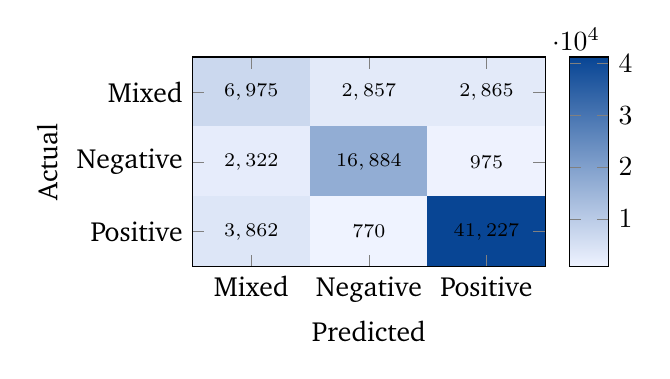
\begin{tikzpicture}
\begin{axis}[
  width=0.50\linewidth,
  height=0.35\linewidth,
  view={0}{90},
  axis on top,
  enlargelimits=false,
  colormap name=myblues, % dùng colormap đã định nghĩa
  colorbar,
  xlabel={Predicted},
  ylabel={Actual},
  xtick={0,1,2},
  ytick={0,1,2},
  xticklabels={Mixed,Negative,Positive},
  yticklabels={Mixed,Negative,Positive},
  y dir=reverse, % để Mixed nằm ở hàng trên cùng
  nodes near coords={
    \pgfmathprintnumber[1000 sep={,}]{\pgfplotspointmeta}
  },
  nodes near coords align=center,
  every node near coord/.append style={
    font=\scriptsize
  },
]
\addplot[
  matrix plot*,
  mesh/cols=3,
  point meta=explicit
] table[meta=z] {
x y z
0 0 6975
1 0 2857
2 0 2865
0 1 2322
1 1 16884
2 1 975
0 2 3862
1 2 770
2 2 41227
};
\end{axis}
\end{tikzpicture}
\caption{Confusion matrix for the LSTM model (test set).}
\label{tab:cm_lstm}
\end{table}

It can be seen that the predicted proportions for Mixed ($16.71\%$ vs. $16.13\%$ actual, $+0.59$ pp) and Negative ($26.05\%$ vs. $25.63\%$, $+0.42$ pp) are slightly overestimated, while Positive ($57.24\%$ vs.\ $58.24\%$) is underestimated by $1.01$ pp. Even though the model classifies the \textit{Positive} class effectively, the matrix highlights significant leakage between \textit{Mixed} and the other two polarities, confirming that the neutral-ambiguous nature of the \textit{Mixed} class remains the primary source of error.

\noindent\textbf{(B) EmbeddingGemma + XGBoost}
\begin{table}[H]
\centering
\small
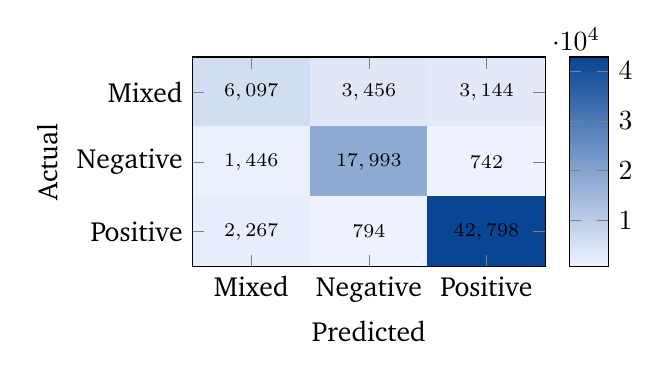
\begin{tikzpicture}
\begin{axis}[
  width=0.50\linewidth,
  height=0.35\linewidth,
  view={0}{90},
  axis on top,
  enlargelimits=false,
  colormap name=myblues, % dùng colormap đã định nghĩa ở preamble
  colorbar,
  xlabel={Predicted},
  ylabel={Actual},
  xtick={0,1,2},
  ytick={0,1,2},
  xticklabels={Mixed,Negative,Positive},
  yticklabels={Mixed,Negative,Positive},
  y dir=reverse,
  nodes near coords={
    \pgfmathprintnumber[1000 sep={,}]{\pgfplotspointmeta}
  },
  nodes near coords align=center,
  every node near coord/.append style={
    font=\scriptsize
  },
]
\addplot[
  matrix plot*,
  mesh/cols=3,
  point meta=explicit
] table[meta=z] {
x y z
0 0 6097
1 0 3456
2 0 3144
0 1 1446
1 1 17993
2 1 742
0 2 2267
1 2 794
2 2 42798
};
\end{axis}
\end{tikzpicture}
\caption{Confusion matrix for the XGBoost model (test set).}
\label{tab:cm_xgboost}
\end{table}

As shown in Table~\ref{tab:cm_xgboost}, the XGBoost model exhibits a conservative bias toward the \textit{Mixed} class, under-predicting its occurrence by $3.67$ pp ($12.46\%$ predicted vs.\ $16.13\%$). This shortfall is largely redistributed to the \textit{Negative} class ($28.25\%$ vs.\ $25.63\%$, $+2.62$ pp) and \textit{Positive} class ($59.29\%$ vs.\ $58.24\%$, $+1.05$ pp). These results suggest that the model tends to default to polarized labels when faced with the high-dimensional complexity of \textit{Mixed} sentiment embeddings.

\noindent\textbf{(C) RoBERTa (fine-tuned)}
\begin{table}[H]
\centering
\small
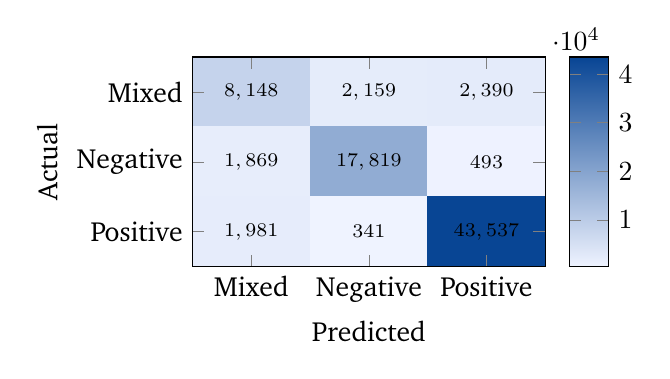
\begin{tikzpicture}
\begin{axis}[
  width=0.50\linewidth,
  height=0.35\linewidth,
  view={0}{90},
  axis on top,
  enlargelimits=false,
  colormap name=myblues,
  colorbar,
  xlabel={Predicted},
  ylabel={Actual},
  xtick={0,1,2},
  ytick={0,1,2},
  xticklabels={Mixed,Negative,Positive},
  yticklabels={Mixed,Negative,Positive},
  y dir=reverse,
  nodes near coords={
    \pgfmathprintnumber[1000 sep={,}]{\pgfplotspointmeta}
  },
  nodes near coords align=center,
  every node near coord/.append style={
    font=\scriptsize
  },
]
\addplot[
  matrix plot*,
  mesh/cols=3,
  point meta=explicit
] table[meta=z] {
x y z
0 0 8148
1 0 2159
2 0 2390
0 1 1869
1 1 17819
2 1 493
0 2 1981
1 2 341
2 2 43537
};
\end{axis}
\end{tikzpicture}
\caption{Confusion matrix for the RoBERTa (fine-tuned) model (test set).}
\label{tab:cm_roberta}
\end{table}

The fine-tuned RoBERTa model achieves the most balanced performance, with a predicted distribution that closely mirrors the ground truth (deviations of $-0.89$ pp for \textit{Mixed}, $+0.18$ pp for \textit{Negative}, and $+0.71$ pp for \textit{Positive}). The resulting matrix demonstrates a significantly sharper diagonal, particularly for the \textit{Mixed} category, indicating that transformer-based attention mechanisms are better equipped to resolve the linguistic nuances that distinguish mixed sentiments from purely positive or negative ones.
\FloatBarrier



\section{Discussion}
In this section, we analyze the specific error patterns of the baseline LSTM model in comparison to the two stronger proposed approaches: fine-tuned RoBERTa and EmbeddingGemma + XGBoost. By examining the subsets of test examples where LSTM fails but the other models succeed, we aim to identify the key weaknesses of the LSTM architecture in handling sentiment classification, particularly for nuanced cases.

Furthermore, we do the same analysis for the two proposed approaches against each other to uncover any complementary strengths or weaknesses. This comparative error analysis provides insights into how different modeling choices impact performance and where future improvements can be targeted.


\subsection{LSTM vs RoBERTa and EmbeddingGemma + XGBoost}

\begin{table}[h]
\centering
\begin{tabular}{lrr}
\hline
True label & Error count & Share of all LSTM errors (\%) \\
\hline
positive & 3{,}124 & 43.03 \\
mixed & 2{,}365 & 32.58 \\
negative & 1{,}771 & 24.39 \\
\textbf{Total} & \textbf{7{,}260} & \textbf{100.00} \\
\hline
\end{tabular}
\caption{Error distribution for the LSTM model on examples where RoBERTa is correct.}
\end{table}

\begin{table}[h]
\centering
\begin{tabular}{lrr}
\hline
True label & Error count & Share of all LSTM errors (\%) \\
\hline
positive & 2{,}830 & 45.45 \\
negative & 1{,}896 & 30.45 \\
mixed & 1{,}500 & 24.09 \\
\textbf{Total} & \textbf{6{,}226} & \textbf{100.00} \\
\hline
\end{tabular}
\caption{Error distribution for the LSTM model on examples where  EmbeddingGemma + XGBoost is correct.}
\end{table}
\FloatBarrier

Key confusion patterns:

\begin{itemize}
  \item \textbf{True \textit{positive} reviews:} In the RoBERTa comparison, 3{,}124 true \textit{positives} are misclassified, with 85.95\% predicted as \textit{mixed} and 14.05\% as \textit{negative}. In the EmbeddingGemma + XGBoost comparison, 2{,}830 true \textit{positives} are misclassified, with 87.07\% predicted as \textit{mixed} and 12.93\% as \textit{negative}.
  \item \textbf{True \textit{negative} reviews:} In the RoBERTa comparison, 1{,}771 true \textit{negatives} are misclassified, with 70.86\% predicted as \textit{mixed} and 29.14\% as \textit{positive}. In the EmbeddingGemma + XGBoost comparison, 1{,}896 true \textit{negatives} are misclassified, with 73.05\% predicted as \textit{mixed} and 26.95\% as \textit{positive}.
  \item \textbf{True \textit{mixed} reviews:} In the RoBERTa comparison, 2{,}365 true \textit{mixed} reviews are misclassified, with 52.39\% predicted as \textit{negative} and 47.61\% as \textit{positive}. In the EmbeddingGemma + XGBoost comparison, 1{,}500 true \textit{mixed} reviews are misclassified, with 52.87\% predicted as \textit{positive} and 47.13\% as \textit{negative}, yielding an almost 50/50 split in both cases.
\end{itemize}

On the subsets of reviews where LSTM failed but the stronger baselines succeeded, LSTM's predictions were distributed as follows:
\begin{itemize}
  \item \textbf{RoBERTa-correct subset:}
  \begin{itemize}
    \item 54.27\% predicted as \textit{mixed}
    \item 23.11\% predicted as \textit{negative}
    \item 22.62\% predicted as \textit{positive}
  \end{itemize}
  \item \textbf{ EmbeddingGemma + XGBoost-correct subset:}
  \begin{itemize}
    \item 61.82\% predicted as \textit{mixed}
    \item 20.94\% predicted as \textit{positive}
    \item 17.23\% predicted as \textit{negative}
  \end{itemize}
\end{itemize}

\textbf{Across both comparisons, LSTM demonstrates a strong over-reliance on the \textit{mixed} label}, applying it to 54.27\% of cases in the RoBERTa subset and 61.82\% of cases in the  EmbeddingGemma + XGBoost subset. This represents a severe miscalibration in handling sentiment nuance: LSTM systematically fails to recognize clearly positive reviews (86--87\% of true \textit{positives} incorrectly classified as \textit{mixed}) and similarly fails to recognize clearly negative reviews (around 71--73\% of true \textit{negatives} defaulted to \textit{mixed}).

\paragraph{Main issue}

The primary failure mode of LSTM is \textbf{systematic over-prediction of the \textit{mixed} sentiment category}, especially when reviews contain any combination of positive and negative language (caveats, minor criticisms, comparisons, acknowledgments of the other side), regardless of the overall sentiment direction. This behavior is consistent across both diagnostic slices (RoBERTa-correct and EmbeddingGemma + Xgboost-correct), indicating a stable structural weakness rather than a comparator-specific artifact.

Concretely, LSTM exhibits three repeating patterns:
\begin{enumerate}
  \item \textbf{Positive $\rightarrow$ Mixed collapse}: it misclassifies $\approx$86--87\% of true \textit{positive} reviews as \textit{mixed} when the review contains even minor criticisms, reservations, or balanced discussion alongside an overall positive stance.
  \item \textbf{Negative $\rightarrow$ Mixed collapse}: it fails to recognize true \textit{negative} reviews $\approx$71--73\% of the time, defaulting to \textit{mixed} when negative sentiment is expressed through measured, analytical language or specific criticisms rather than purely emotional condemnation, and when the reviewer acknowledges small positives.
  \item \textbf{Mixed $\rightarrow$ Forced polarity}: for genuinely mixed reviews, LSTM fails to detect the balanced nature that defines the class and instead splits them nearly evenly into \textit{positive} vs \textit{negative} (roughly 50/50), suggesting it detects opposing signals but cannot represent ``balance'' as its own decision.
\end{enumerate}

Overall, LSTM appears to treat sentiment as a shallow aggregation of positive/negative tokens, while RoBERTa and EmbeddingGemma + Xgboost successfully capture contextual weighting, rhetorical structure, and overall argumentative flow. LSTM struggles to distinguish:
\begin{itemize}
  \item ``good but with flaws'' (positive),
  \item ``strengths and weaknesses are roughly balanced'' (mixed),
  \item ``bad despite some redeeming qualities'' (negative).
\end{itemize}

\paragraph{How this problem manifests}

LSTM’s over-reliance on \textit{mixed} predictions manifests in several specific ways:

\begin{itemize}
\item \textbf{For true \textit{positive} reviews:}
LSTM is triggered into predicting \textit{mixed} by any mention of flaws, limitations, caveats, or comparisons, even when these are minor relative to overall praise. Reviews that acknowledge weaknesses while concluding with a clear recommendation are systematically misclassified. The model struggles to separate ``positive with honest assessment'' from ``genuinely balanced mixed.''

\item \textbf{For true \textit{negative} reviews:}
When negative reviews use measured or analytical language (``the gameplay is slow and very basic… the biggest problem is…'') or acknowledge small positives while maintaining an overall negative stance, LSTM often defaults to \textit{mixed}. It can also be vulnerable to tone or rhetorical tricks (e.g., sarcasm/irony) where surface-level phrasing does not match the underlying sentiment intent.

\item \textbf{For genuinely mixed reviews:}
LSTM fails to recognize balanced sentiment as its own category. Instead, it forces nuanced reviews into binary \textit{positive} or \textit{negative} buckets almost randomly (approximately 50/50 split). Reviews with explicit balancing cues (e.g., ``mixed bag,'' structured PROS/CONS, or evenly weighted trade-offs) are misclassified because LSTM cannot integrate competing sentiments into a stable ``balanced'' decision.

\end{itemize}
The underlying issue is that LSTM detects mixed signals but fails to integrate them into a coherent global assessment, unlike RoBERTa and EmbeddingGemma + Xgboost which successfully navigate the same nuanced cases.

\paragraph{Practical implications}

\begin{itemize}
  \item \textbf{Production risk: biased sentiment distribution.} Using the LSTM in a game-review sentiment pipeline would materially distort outputs, especially due to systematic over-prediction of \textit{Mixed} (by roughly 54--62\% across both comparisons).

  \item \textbf{False-neutral ``sentiment void''.} Many genuinely \textbf{Positive} reviews (useful for recommendations and conversions) and clearly \textbf{Negative} reviews (useful for quality monitoring and alerts) are diluted into an ambiguous middle class that is less actionable.

  \item \textbf{Error composition is business-relevant.} In the XGBoost comparison, about \textbf{45\%} of the LSTM's errors are missed positives and about \textbf{30\%} are missed negatives, implying:
    \begin{itemize}
      \item loved games are under-surfaced (weaker discovery/recommendation signals),
      \item problematic releases are insufficiently flagged (weaker QA / trust-and-safety signals).
    \end{itemize}

  \item \textbf{Unreliable aggregate metrics on high-value content.} Sentiment summaries derived from the LSTM become least trustworthy on nuanced, thoughtful reviews.

  \item \textbf{Architecture implication.} Since both RoBERTa and EmbeddingGemma + XGBoost handle these same cases better, the LSTM setup here appears ill-suited for document-level sentiment:
    \begin{itemize}
      \item it likely follows local word-level polarity shifts without integrating them into a stable global judgment,
      \item stronger baselines better exploit contextual cues and feature interactions to resolve ambiguity.
    \end{itemize}
\end{itemize}



\subsection{EmbeddingGemma + XGBoost vs RoBERTa}

\begin{table}[H]
\centering
\begin{tabular}{lrr}
\hline
True label & Error count & Share of all XGBoost errors (\%) \\
\hline
mixed & 2{,}875 & 53.51 \\
positive & 1{,}602 & 29.81 \\
negative & 896 & 16.68 \\
\textbf{Total} & \textbf{5{,}373} & \textbf{100.00} \\
\hline
\end{tabular}
\caption{XGBoost errors on examples where RoBERTa is correct.}
\end{table}

Key confusion patterns:

\begin{itemize}
  \item \textbf{True \textit{mixed} (2{,}875 errors)}: 57.18\% predicted as \textit{negative}, 42.82\% as \textit{positive}
  \item \textbf{True \textit{positive} (1{,}602 errors)}: 76.03\% predicted as \textit{mixed}, 23.97\% as \textit{negative}
  \item \textbf{True \textit{negative} (896 errors)}: 72.66\% predicted as \textit{mixed}, 27.34\% as \textit{positive}
\end{itemize}

On reviews where EmbeddingGemma +  XGBoost failed but RoBERTa succeeded, embeddingGemma's predictions were:

\begin{itemize}
  \item 37.74\% \textit{negative}
  \item 34.79\% \textit{mixed}
  \item 27.47\% \textit{positive}
\end{itemize}

\textbf{EmbeddingGemma + Xgboost shows a relatively balanced distribution across categories}, but critically fails on genuinely \textit{mixed} reviews, misclassifying them as binary sentiments 100\% of the time. This represents the model's primary weakness: complete inability to recognize balanced sentiment.


\paragraph{Main issue}

The primary failure mode of EmbeddingGemma + Xgboost is its \textbf{catastrophic inability to correctly identify genuinely \textit{mixed} reviews}, which account for 53.51\% of all its errors. Unlike LSTM which over-predicts \textit{mixed}, embeddingGemma does the opposite: it forces genuinely balanced reviews into binary \textit{positive} (43\%) or \textit{negative} (57\%) categories, unable to recognize when a review expresses balanced criticism or praise. For true \textit{positive} and negative reviews, the model shows a secondary failure pattern of over-predicting \textit{mixed} (76\% and 73\% respectively), but this is less severe than its complete failure on actual mixed sentiment. The model appears to use a simplistic decision boundary: if it detects both positive and negative signals and one seems slightly dominant, it classifies to that extreme; if signals seem equally balanced, it defaults to \textit{mixed} even when the overall sentiment is clearly positive or negative. This suggests the embedding-based approach captures semantic similarity but lacks the nuanced contextual understanding needed to weigh competing sentiments and detect genuine balance versus qualified positive/negative sentiment.

\paragraph{How this problem manifests}

\begin{itemize}
\item \textbf{For true \textit{mixed} reviews}, EmbeddingGemma +  Xgboost completely fails to recognize balanced sentiment, instead forcing every genuinely mixed review into either \textit{positive} or \textit{negative} categories. Reviews with explicit PROS/CONS structure, phrases like ``mixed bag,'' or statements like ``not as good as... but still decent'' are systematically misclassified. For example, a review about Senran Kagura stating ``mechanics are pretty decent... however missions are incredibly boring... not the worst game... but missions structure is boring and repetitive'' is classified as \textit{negative} when it's clearly expressing balanced mixed sentiment. Similarly, a detailed review of SWTOR stating ``deeply flawed, incredibly addictive... The story is great, but game mechanics are a deal-killer. Cautiously recommend'' is misread as \textit{positive} despite explicitly stating mixed feelings. The model cannot detect the rhetorical markers of balanced criticism.



\item \textbf{For true \textit{positive} reviews}, embeddingGemma defaults to \textit{mixed} when reviews contain any negative language or qualifications, even when the overall recommendation is clearly positive. Reviews stating ``pretty good. If you're an old Spyro fan... you will enjoy this'' are misclassified as \textit{mixed} because the model detects the qualification ``if'' and interprets minor reservations as balanced criticism. Reviews praising games while acknowledging limitations like ``good but not perfect'' or ``I enjoyed it despite some flaws'' trigger the \textit{mixed} classification incorrectly.


\item \textbf{For true \textit{negative} reviews}, embeddingGemma similarly over-predicts \textit{mixed} when negative reviews contain any positive acknowledgments or measured language. A scathing Silent Hill HD Collection review explaining in detail why it's terrible but framed as an analytical comparison (``if we were reviewing SH2 and 3 you'd see nines and tens, this however...'') is misclassified as \textit{positive}, showing the model's inability to track negation and contrastive rhetoric. Reviews using phrases like ``Flaming pile of ****'' but followed by explanatory context are classified as \textit{mixed} when the sentiment is unambiguously negative.


\end{itemize}

\paragraph{Root cause analysis}

The underlying issue is that EmbeddingGemma + Xgboost, despite its semantic embedding capabilities, lacks the sophisticated contextual reasoning that RoBERTa's transformer architecture provides. It cannot properly aggregate competing sentiments, track rhetorical flow, or distinguish between ``qualified positive,'' ``genuinely balanced mixed,'' and ``acknowledged negative.''



\paragraph{Practical implications}

\begin{itemize}
  \item \textbf{High deployment risk for nuanced sentiment.} The model largely fails to correctly identify genuinely \textit{Mixed} reviews; around \textbf{53\% of all errors} are due to Mixed cases, so it is not reliable when nuance is required.

  \item \textbf{False-binary behavior (loss of nuance).} Instead of producing a false-neutral middle (as with the LSTM), EmbeddingGemma +  Xgboost tends to force balanced reviews into \textbf{Positive} or \textbf{Negative}, collapsing the most informative feedback (both pros and cons) into extreme labels.

  \item \textbf{Impact on developer/publisher insight.} Because mixed reviews often contain the most actionable detail (what works vs.\ what breaks), this failure directly reduces the usefulness of sentiment analytics for prioritizing fixes and improvements.

  \item \textbf{Noise from class imbalance in predictions.} For \textbf{Positive} and \textbf{Negative} reviews, the model's reported \textbf{76\%} and \textbf{73\%} over-prediction of \textit{Mixed} adds noise to aggregate reporting, though it is less damaging than the Mixed-class failure itself.

  \item \textbf{Rhetorical/linguistic vulnerability.} Weak handling of \textbf{negation} and \textbf{contrastive rhetoric} (e.g., “good idea, but terrible execution”) can produce harmful errors, including cases where strongly negative reviews are misclassified as \textbf{Positive}.
\end{itemize}

\section{Conclusion}

\noindent \textbf{Project Summary} This project successfully established an end-to-end pipeline for sentiment analysis in the video game domain. The team constructed a robust benchmark dataset of 629,884 reviews scraped from Metacritic to address the unique linguistic challenges of gaming feedback, such as slang ("nerf," "buff") and sarcasm. Three distinct modeling approaches were implemented and evaluated: a baseline Bidirectional LSTM, a fine-tuned RoBERTa transformer, and a hybrid approach using EmbeddingGemma + XGBoost classification.

\vspace{1em}

\noindent \textbf{Key Findings} The comparative analysis revealed a distinct trade-off between predictive performance and computational efficiency:

\begin{itemize}
    \item \textbf{Best Overall Performance (RoBERTa):} The fine-tuned RoBERTa model proved to be the superior architecture for understanding semantic nuance. It achieved the highest global metrics (Accuracy: 88.27\%, Macro F1: 0.8278) and demonstrated the "cleanest separation" between classes. It was particularly effective at identifying "Mixed" reviews, a category where other models struggled significantly.
    
    \item \textbf{Best Efficiency (EmbeddingGemma + XGBoost):} This hybrid approach offered a strong middle ground. It drastically reduced training time (approx. 9 minutes compared to RoBERTa's $\sim$31 hours) while maintaining competitive accuracy (84.95\%). However, it suffered from a "false-binary" behavior, where it failed to recognize nuanced "Mixed" sentiment, forcing those reviews into Positive or Negative categories.
    
    \item \textbf{Highest Throughput (LSTM):} While the LSTM baseline lagged in predictive quality (Accuracy: 82.66\%) and suffered from a "false-neutral" bias (often misclassifying clear opinions as Mixed), it offered the highest inference speed ($\sim$1,913 samples/second), making it potentially useful for high-volume, real-time streams where depth of understanding is secondary.
\end{itemize}

\vspace{1em}

\noindent \textbf{Final Verdict} The study concludes that while dense embedding approaches (EmbeddingGemma + XGBoost) provide a viable, resource-efficient alternative for general sentiment classification, \textbf{fine-tuned Transformers (RoBERTa) remain essential for capturing the complex, nuanced opinions} typical of the gaming community. Future work could focus on improving the efficiency of the Transformer model or addressing the specific inability of the embedding-based model to detect balanced, mixed sentiments.


\section{Group Contributions \& Resources}
\subsection{Group Contributions}

\begin{table}[h!]
    \centering
    \renewcommand{\arraystretch}{1.4} % Vertical spacing
    
    % Adjusted column width to p{8cm} to fit descriptions better
    \begin{tabular}{@{} l c p{8cm} @{}} 
        \toprule
        \textbf{Name} & \textbf{Student ID} & \textbf{Contributions} \\
        \midrule
        Au Trung Phong & 20225455 & Team Leader, Data Preparation, System Refinement \\
        Nguyen Nam Khanh & 20225448 & LSTM Baseline Implementation, Data Analysis \\
        Vu Duc Minh & 20225514 & Final Result Analysis \\
        Tran Sy Minh Quan & 20225521 & RoBERTa Approach Implementation \\
        Bui Van Huy & 20225497 & Dense Embedding + XGBoost Implementation \\
        \bottomrule
    \end{tabular}
    \caption{Group Members and Contributions}
    \label{tab:contributions}
\end{table}

\subsection{Resources}
\begin{enumerate}
    \item \textbf{Source Code:} \href{https://github.com/auphong2707/sentiment-analysis-for-game-review}{GitHub Repository}
    \item \textbf{Dataset:} \href{https://huggingface.co/datasets/auphong2707/game-reviews-sentiment}{HuggingFace Dataset}
    \item \textbf{Final Models:}
        \begin{itemize}
            \item LSTM Baseline: \href{https://huggingface.co/auphong2707/wm-grsa-lstm-baseline-results}{Model Link}
            \item Embedding Gemma + XGBoost: \href{https://huggingface.co/auphong2707/wm-grsa-eg-xgboost-results}{Model Link}
            \item Finetuned RoBERTa: \href{https://huggingface.co/auphong2707/wm-grsa-roberta-softmax-results}{Model Link}
        \end{itemize}
    \item \textbf{Kaggle Training Sessions:}
        \begin{itemize}
            \item LSTM Baseline: \href{https://www.kaggle.com/code/phongau/sentiment-analysis-for-game-review/output?scriptVersionId=287967429}{Session Log}
            \item Embedding Gemma + XGBoost:
                \begin{enumerate}
                    \item \href{https://www.kaggle.com/code/phongau/wm-xgboost/output?scriptVersionId=288046131}{Part 1}
                    \item \href{https://www.kaggle.com/code/thesyx03/wm-xgboost-continue/output?scriptVersionId=288146195}{Part 2 (Continued)}
                \end{enumerate}
            \item Finetuned RoBERTa:
                \begin{enumerate}
                    \item \href{https://www.kaggle.com/code/veilwings/roberta-sentiment-analysis/output?scriptVersionId=287976438}{Part 1}
                    \item \href{https://www.kaggle.com/code/veilwings/roberta-sentiment-analysis-cont/output?scriptVersionId=288149370}{Part 2}
                    \item \href{https://www.kaggle.com/code/veilwings/roberta-sentiment-analysis-cont-cont/output?scriptVersionId=288290606}{Part 3}
                    \item \href{https://www.kaggle.com/code/justveil/roberta-sentiment-analysis-cont-cont-cont/output?scriptVersionId=288398950}{Part 4}
                \end{enumerate}
        \end{itemize}
\end{enumerate}


\bibliographystyle{plain}  % Sets style to numbered [1], [2]
\bibliography{main}


\end{document}

